%%%%%%%%%%%%%%%%%%%%%%%%%%%%%%%%%%%%%%%%%
% Reporte con clase
% J. Santander 
% Versión 1.4.5 (3/6/15)
% Licencia: by-nc-sa
%%%%%%%%%%%%%%%%%%%%%%%%%%%%%%%%%%%%%%%%%

\documentclass[11pt, a4paper, twosides]{report}
\usepackage[a4paper]{geometry}
\geometry{verbose,tmargin=4cm,bmargin=3cm,lmargin=3cm,rmargin=3cm}
\usepackage[spanish,es-tabla]{babel}
\usepackage{appendix}

% Lenguaje y codificación:
\usepackage{lettrine}
\usepackage[T1]{fontenc}
\usepackage[utf8]{inputenc}
%\newcommand*\initfamily{\usefont{U}{Kramer}{xl}{n}}
\usepackage{changepage}
\usepackage{ragged2e}

% Fuentes:
\usepackage{eulervm}
%\usepackage[scaled]{helvet} %Helvetica
\usepackage{charter}
\usepackage{blindtext, color}
\usepackage[compact]{titlesec}
\usepackage{tocloft}

\renewcommand*\sfdefault{pag}
\fontfamily{phv}

\newcommand{\hsp}{\hspace{20pt}}
\titleformat{\chapter}[hang]{\Huge\bfseries}{\thechapter\hsp\textcolor{gray75}{|}\hsp}{0pt}{\Huge\bfseries}

\titleformat{\section}[hang]{\fontfamily{phv}\selectfont\bfseries}{\thesection\hsp}{0pt}{}{}
\titleformat{\subsection}[hang]{\fontfamily{phv}\selectfont}{\thesubsection\hsp}{0pt}{}{}
\titleformat{\subsubsection}[hang]{\fontfamily{phv}\selectfont\itshape}{\hsp}{0pt}{}{}

\setcounter{tocdepth}{1}
\renewcommand{\cftdot}{\textcolor[gray]{0.75}{--}}
\renewcommand{\cftdotsep}{0}

\renewcommand{\cftchapfont}{\fontfamily{phv}\selectfont\bfseries}

\addto\captionsspanish{\renewcommand{\contentsname}{\huge\fontfamily{phv}\selectfont{Índice de contenidos}}}
\addto\captionsspanish{\renewcommand{\listfigurename}{\huge\fontfamily{phv}\selectfont{Índice de figuras}}}
\addto\captionsspanish{\renewcommand{\listtablename}{\huge\fontfamily{phv}\selectfont{Índice de tablas}}}

\titleformat{\chapter}[hang]{\Huge\fontfamily{phv}\selectfont}{\thechapter\hsp{\textcolor{gray75}{\rule[-0.75ex]{0.08ex}{1.5em}}}\hsp}{0pt}{\huge\bfseries}{}

% Matemáticas
\usepackage{mathtools}
\usepackage{amsmath}
\usepackage{amsfonts}
\usepackage{tabu}
\usepackage{amsthm}

\newcolumntype{L}[1]{>{\raggedright\let\newline\\\arraybackslash\hspace{0pt}}m{#1}}
\newcolumntype{C}[1]{>{\centering\let\newline\\\arraybackslash\hspace{0pt}}m{#1}}
\newcolumntype{R}[1]{>{\raggedleft\let\newline\\\arraybackslash\hspace{0pt}}m{#1}}

% Color, gráficas e hiper
\usepackage{xcolor, colortbl}
\usepackage{graphicx}
\usepackage{hyperref}
\hypersetup{
	colorlinks=true,       %Activar color de los links
	linkcolor=darkblue,    %Referencias cruzadas
	citecolor=darkblue,    %Citas bibliográficas
	filecolor=blue,        %Referencias internas
	urlcolor=darkgreen     %Referencias externas
}
\definecolor{gray75}{gray}{0.75}                        %Color gris
\definecolor{mygreen}{RGB}{28,172,0}                    %Color Verde
\definecolor{mylilas}{RGB}{170,55,241}                  %Color lila
\definecolor{myorange}{rgb}{1.0,0.4,0}                  %Color Naranja
\definecolor{myred}{rgb}{0.698039,0.133333,0.133333}    %Color rojo
\definecolor{darkblue}{RGB}{0,0,90}
\definecolor{darkgreen}{RGB}{0,80,0}

%Bibliografía
\usepackage{biblatex}
\bibliography{SC.bib}

\DeclareCiteCommand{\cite}[\mkbibfootnote]
{\usebibmacro{prenote}}{
    \usebibmacro{citeindex}
    \mkbibbrackets{\usebibmacro{cite}}
    \setunit{\addnbspace}
    \printnames{author}
    \setunit{\labelnamepunct}
    \printfield{journaltitle}
    \newunit
    \printfield{year}
}
{\addsemicolon\space}
{\usebibmacro{postnote}}

\DeclareFieldFormat[article]{year}{(#1)}
\DefineBibliographyStrings{spanish}{andothers={\emph{et al}\adddot}}

\DeclareBibliographyDriver{article}{
\usebibmacro{bibindex}
\usebibmacro{begentry}
\newunit\newblock
\printnames{author}
\newunit\newblock
\usebibmacro{journal}
\newunit\newblock
\printfield{volume}
\newunit\newblock
\printfield{number}
\newunit\newblock
\usebibmacro{note+pages}
\newunit\newblock
\printfield{year}
\newunit\newblock
\usebibmacro{pageref}
\newline\newblock
\printfield{title}
{\iffieldundef{doi}{
    {\iffieldundef{url}
    {}
    {\newline\newblock
    \usebibmacro{doi+eprint+url}}
    {}
    }
}
{\newline\newblock
\usebibmacro{doi+eprint+url}}
{}
}
\finentry}

\renewbibmacro*{doi+eprint+url}{
\iftoggle{bbx:doi}
{\iffieldundef{url}{\printfield{doi}}{}}{}
\iftoggle{bbx:eprint}
{\iffieldundef{doi}{\usebibmacro{eprint}}{}}{}
\iftoggle{bbx:url}
{\usebibmacro{url+urldate}}{}
}

%Remover espacio en blanco de capítulos
\makeatletter
\def\ttl@mkchap@i#1#2#3#4#5#6#7{%
    \ttl@assign\@tempskipa#3\relax\beforetitleunit
    \vspace{\@tempskipa}
    \global\@afterindenttrue
    \ifcase#5 \global\@afterindentfalse\fi
    \ttl@assign\@tempskipb#4\relax\aftertitleunit
    \ttl@topmode{\@tempskipb}{%
        \ttl@select{#6}{#1}{#2}{#7}}%
    \ttl@finmarks  
    \@ifundefined{ttlp@#6}{}{\ttlp@write{#6}}}
\makeatother

%Fuentes de las figuras:
\usepackage{epstopdf}
\usepackage{lipsum}       % Lorem ipsum
\graphicspath{{Figuras/}} % Carpeta de las figuras
\usepackage[format=hang]{caption}
\renewcommand{\captionlabelfont}{\fontfamily{phv}\selectfont\bfseries\small}

%Cabeceras
\usepackage{fancyhdr}
\pagestyle{fancy}

\fancyhead[RO]{\fontfamily{phv}\selectfont \nouppercase\rightmark}
                \renewcommand{\sectionmark}[1]{\markright{\arabic{chapter}.\arabic{section} \, #1}}
\fancyhead[LO]{\fontfamily{phv}\selectfont Proyecto de servicio comunitario 2016}

%Fuentes para tablas
\usepackage{tabularx}
\usepackage{multirow}
\usepackage{float}
\usepackage{subfig}
\makeatletter
  \def\Hv@scale{.95}
\makeatother
\DeclareRobustCommand{\tablefont}{%
        \fontencoding{\encodingdefault}%
        \fontseries{m}
        \fontshape{n}
        \fontfamily{phv}
        \fontsize{9}{12}
        \selectfont}
\DeclareTextFontCommand{\texttable}{\tablefont}
        
%interlineado
\linespread{1.22}
\setlength{\parskip}{\baselineskip}%
\setlength{\parindent}{1em}%

%Apéndices
\renewcommand{\appendixname}{\Huge\fontfamily{phv}\selectfont{Apéndices}}
\renewcommand{\appendixtocname}{Apéndices}
\renewcommand{\appendixpagename}{\Huge\fontfamily{phv}\selectfont{Apéndices}}

\begin{document}

%%%%%%%%%%%%%% PORTADA %%%%%%%%%%%%%%%%%%%%%%%%%%%%%%%
    \begin{titlepage}
        \newcommand{\HRule}{\rule{\linewidth}{0.5mm}} 
        \begin{center} % Centrar todo
        \noindent
        \begin{minipage}[b]{0.14\textwidth}    
            
\includegraphics[width=1.5cm]{loguc.png}
        \end{minipage}%
        \begin{minipage}[b][2cm]{0.6\textwidth}
            \centering\
            UNIVERSIDAD DE CARABOBO \vfill
            FACULTAD DE INGENIERÍA \vfill
            ESCUELA DE TELECOMUNICACIONES \vfill
            PROYECTO DE SERVICIO COMUNITARIO
        \end{minipage}%
        \begin{minipage}[b]{0.2\textwidth}
            
\includegraphics[width=3cm]{Logfac.png}
        \end{minipage}\\ [3cm] 
        
        {\Large  \sf  Diseño de un Enlace de Microondas entre el Núcleo San Diego de la Dirección de Extensión y Servicio Comunitario y la Dirección de Medios Electrónicos y Telemática de la Universidad de Carabobo }\\[1.5cm]           %Titulo del documento
        \end{center}
        \begin{minipage}{0.5\textwidth}
            \begin{flushleft} \small
               \emph{Tutores:}\\      %Tutores
                Prof. Ing. P. Del Pino \\
                Prof. Ing. C. Aponte
            \end{flushleft}
        \end{minipage}
        ~
        \begin{minipage}{0.5\textwidth}
            \begin{flushright} \small
               \emph{Autores:} \\   
               Equipo de servicio comunitario 2016 \\de la Escuela de Ingeniería de Telecomunicaciones%Autores 
            \end{flushright}
        \end{minipage}
        {\justify \noindent \center{\large{\textbf{Resumen}}}\\
           El siguiente proyecto de servicio comunitario presentado ante la escuela de ingeniería de telecomunicaciones de la Universidad de Carabobo consiste en el diseño de un sistema que proporcionará servicios de telefonía e Internet a la dependencia Dirección de Extensión y Servicios a la Comunidad (DESCO) núcleo San Diego. Para este diseño se tomaron en cuenta los siguientes aspectos: ubicación de la torre de telecomunicaciones, sistemas de protección, equipos, materiales necesarios, planificación de la red y recomendaciones para la ejecución del proyecto. Al disponer de Internet la DESCO-San Diego podrá dictar un mayor número de cursos relacionado con la computación a la comunidad, además de poder brindar un mejor servicio.}
           
           {\noindent{\large{\textbf{Palabras clave}}}: Cableado estructurado, planificación de redes, comunicaciones}\\[1.5cm]
        
        \center{{\small \today}}
    \end{titlepage}

{\pagestyle{plain}
\tableofcontents
\newpage
\listoffigures
\newpage 
\listoftables
\cleardoublepage}

%%%%%%%%%%% INTRODUCCIÓN %%%%%%%%%%%%%%%%%%%%%%%%%%%%%%%%%%%%%
\chapter{Introducción}
En el mes de Agosto de 2015, se le presenta como Proyecto de Servicio Comunitario a la Escuela de Telecomunicaciones una problemática que tiene la Dirección de Extensión y Servicio Comunitario (\textbf{DESCO}) ubicada en la Urbanización El Tulipán, entre las parcelas 5 y 9, San Diego, Estado Carabobo y la Dirección de Medios Electrónicos y Telemática (\textbf{DIMETEL}) ubicada en los recintos de la Universidad de Carabobo. Dicha problemática consiste en la falta de comunicación que existe entre ambos lugares y la necesidad de acceso a internet para la \textbf{DESCO}.

Un grupo de Estudiantes de la Escuela de Telecomunicaciones destinados a la realización de dicho Servicio Comunitario, coordinados por los Profesores Carlos Aponte y Paulino Del Pino proceden a idear una solución, que consiste en la realización de un radioenlace de microondas entre los núcleos de \textbf{DIMETEL} y la \textbf{DESCO}, cuya ejecución se fracciono en las siguientes etapas:

\begin{itemize}
    \item Designación de Equipos.
    \item Visitas Informativas.
    \item Asignación de Tópicos Técnicos.
    \item Desarrollo de Tópicos Técnicos.
    \item Discusión de Tópicos Técnicos.
    \item Entrega Final de Proyecto.
\end{itemize}

El proyecto que se presenta a continuación será implementado por la Dirección De Medios Electrónicos y Telemática (\textbf{DIMETEL}), sin embargo, el financiamiento se logrará gracias a los recursos de la Universidad de Carabobo.

El propósito de dicha labor se basa en que la \textbf{DESCO} cuente con servicio a internet, logrando que los trabajadores realicen todas sus labores de manera efectiva en su sitio de trabajo, además de modernizar la institución en la nueva era informativa, logrando captar la atención y la integración de la comunidad en todos los cursos que propone dicha institución, fomentando el desarrollo de la educación y las artes en los jóvenes y adultos.


%%%%%%%%%%% LISTADO DE ESTUDIANTES %%%%%%%%%%%%%%%%%%%%%%%%%%%
\chapter{Identificación de los participantes}

\begin{table}[ht]
\centering
\scalebox{0.75}{\begin{tabular}{ | l | l | l | l | l | l | }
\hline
\cellcolor{gray75}	Cédula & \cellcolor{gray75} Apellido &\cellcolor{gray75} Nombre & \cellcolor{gray75} Escuela &\cellcolor{gray75} Correo &\cellcolor{gray75} Responsabilidad \\ \hline
	21479512 & Cabrera & Pedro & Telecomunicaciones & pedrom9632@gmail.com & Redacción \  \\ \hline
	19218886 & Canelon & Francisco & Telecomunicaciones & canelonfransico@gmail.com & Redacción  \  \\ \hline
	20727066 & Coronel & Mael & Telecomunicaciones & alejandroing152010@gmail.com & Integración \  \\ \hline
	20480492 & Díaz & Anderson & Telecomunicaciones & adjmxx2015@gmail.com & Integración \  \\ \hline
	19973194 & Escalona & Hecmar & Telecomunicaciones & hecmarescalona@hotmail.com & Ejecución \  \\ \hline
	23572093 & Fernandez & Robert & Telecomunicaciones & fernandezrobert15@gmail.com & Ejecución \  \\ \hline
	23587800 & Gamboa & Antonio & Telecomunicaciones & antoniojg92@gmail.com & Redacción\  \\ \hline
	19697560 & Gomez & Leoncio & Telecomunicaciones & lncgomz@gmail.com & Ejecución\  \\ \hline
	22696801 & González & Samuel & Telecomunicaciones & sam110494@hotmail.com  & Supervisión \  \\ \hline
	20030984 & Henriquez & Dahunaharany & Telecomunicaciones & dahu\_hquez@hotmail.com & Supervisión\  \\ \hline
	22610475 & Herrera & Josefa & Telecomunicaciones & herreraclaudia28@gmail.com  & Supervisión \  \\ \hline
	20758835 & Herrera & Jose & Telecomunicaciones & jdhgraterol@gmail.com & Ejecución \  \\ \hline
	20663877 & Noguera & Alirio & Telecomunicaciones & alnog1507@gmail.com &  Ejecución\  \\ \hline
	20467639 & Nuñez & Jhoander & Telecomunicaciones & jhoandern@gmail.com & Redacción \  \\ \hline
	21019407 & Perretti & Giusseppe & Telecomunicaciones & gperretti\_207@hotmail.com & Redacción \  \\ \hline
	21216712 & Ríos & Pedro & Telecomunicaciones & peterivers108@gmail.com & Ejecución\  \\ \hline
	20591860 & Rudolf & Rosanna & Telecomunicaciones & rosannarudolf@gmail.com & Ejecución\  \\ \hline
	20757380 & Sanchez & Crisanto & Telecomunicaciones & crisanto.sanchezp@gmail.com & Integración \  \\ \hline
	20523854 & Sanchez & Norelia & Telecomunicaciones & nore.sc.19@gmail.com & Redacción\  \\ \hline
	24444598 & Santander & Jesus & Telecomunicaciones & jesusg33@gmail.com & Integración\  \\ \hline
\end{tabular}}
\label{tab:AntC}
\end{table}

%%%%%%%%%%% DIAGNOSTICO %%%%%%%%%%%%%%%%%%%%%%%%%%%%%%%%%%%%%%%
\chapter{Diagnostico de la situación actual}
 En la etapa de Visitas Informativas se logró determinar que la Dirección de Extensión y Servicio Comunitario (\textbf{DESCO}), ha logrado detectar las necesidades que padece la comunidad, las cuales son:
 
\begin{itemize}
    \item Problemas de Integración entre los ciudadanos.
    \item Problemas de Oratoria.
    \item Escases de Arte y Cultura
    \item Problemas de Esparcimiento.
\end{itemize}

Las causas de dichas necesidades corresponden a la falta de personal y zonas en donde los ciudadanos puedan educarse, compartir y recrearse, incentivando a los jóvenes y adultos al sano esparcimiento y desarrollo del arte.

La \textbf{DESCO} ofrece servicios que disminuyen las carencias de dicha comunidad, brindando talleres y un espacio para la integración, además la misma funciona como centro de acopio para la asistencia de otras comunidades que atraviesen una situación de auxilio. Desde la existencia de la institución, las necesidades que presenta la comunidad han disminuido notablemente, sin embargo, el no disponer servicio de internet reduce el rango de usuarios que visita y conoce la institución e internamente dificulta el desempeño del personal de la DESCO.

La institución cuenta con los recursos de: espacio para la educación, áreas verdes para la recreación y un excelente personal capacitado para el manejo de los servicios que ofrecen.

\newpage
\section{Árbol de problemas}

\begin{figure}[H]
    \centering
    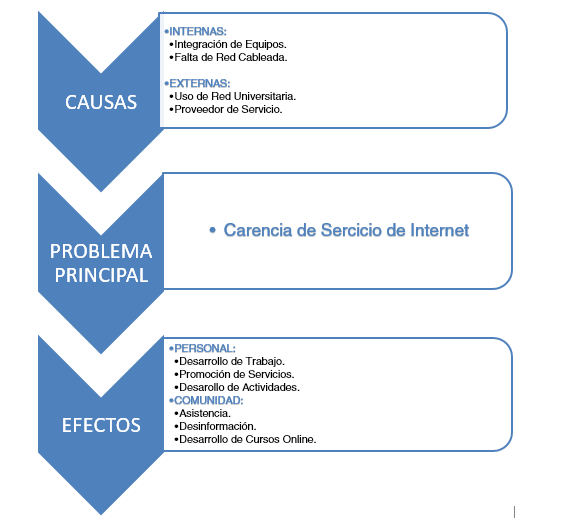
\includegraphics[width= 1 \linewidth]{a.png}
    \caption{Árbol de problemas}
    \label{fig:problem_tree}
\end{figure}

%%%%%%%%%%% JUSTIFICACIÓN %%%%%%%%%%%%%%%%%%%%%%%%%%%%%%%%%%%%%%%

\chapter{Justificación}
Las telecomunicaciones son una herramienta importante en la actualidad, las cuales cumplen un propósito fundamental; mejorando la efectividad en el desempeño de las diversas actividades que se lleven a cabo en instituciones. Actualmente, en la Dirección de Extensión y Servicio Comunitario de la Universidad de Carabobo (DESCO), Núcleo San Diego; existe la limitación tanto en el desempeño de sus funciones laborales como en la ejecución y ampliación de sus servicios, esto debido a la no disponibilidad de una red de telecomunicaciones en la institución. Por esta razón, la motivación de la Escuela de Ingeniería en Telecomunicaciones para el desarrollo del Proyecto de Servicio Comunitario titulado <<Diseño de un Enlace de Microondas entre el Núcleo San Diego de la Dirección de Extensión y Servicio Comunitario y la Dirección de Medios Electrónicos y Telemática de la Universidad de Carabobo >>, proporcionando una solución que una vez implementada, permitirá la ejecución y ampliación efectiva de las actividades y servicios prestados por dicha institución, beneficiando así, tanto al personal de DESCO (Núcleo San Diego) y a la comunidad de San Diego

%%%%%%%%%%% DELIMITACIÓN %%%%%%%%%%%%%%%%%%%%%%%%%%%%%%%%%%%%%%%%%%%
\chapter{Delimitación}
El proyecto tiene  el propósito de permitirle a la Dirección de Extensión y  Servicios a la Comunidad (DESCO) ubicado en la Urbanización Tulipán del municipio de San Diego, poseer servicios de internet en el municipio San Diego del estado Carabobo a través del radio enlace  cerro La Cruz- Tulipán. Donde el periodo de ejecución del Proyecto tuvo fecha de inicial del 5 de agosto de 2015 hasta \textbf{DÍA} agosto de 2016, siendo la fecha de inicial la primera visita que se realizó al sitio ya mencionado. 

Este proyecto tiene un impacto positivo en los empleados  ubicados en la DESCO del municipio ya mencionado, en donde  podrán realizar las actividades en su lugar  de trabajo que requiera servicios de internet, además también posee un impacto positivo en la comunidad  ya que se puede ofrecer una  mejor calidad en cursos, charlas, etc., adicionalmente en un futuro podrían ofrecer servicios de internet o cursos on-line a través de una sala telemática instalada  en  estos espacios,  el proyecto va de la mano con la Dirección de Medios Electrónicos y Telemática de la Universidad de Carabobo (DIMETEL), el cual tienen la capacidad de llevar acabo la ejecución del proyecto. 

La instalación de los equipos solo se realizara solo en la DESCO debido a que ya se cuenta con los equipos necesarios en cerro La Cruz, lo cual esto representa un impacto mínimo  en el ambiente ya que para la instalación \textbf{de estos equipos se necesitara hacer excavaciones pequeñas en el terreno de la DESCO}. 

%%%%%%%%%%% OBJETIVOS %%%%%%%%%%%%%%%%%%%%%%%%%%%%%%%%%%%%%%%%%%%

\chapter{Objetivos}

\section{Objetivo especifico}
Diseñar un enlace de microondas entre el Núcleo ubicado en San Diego de la Dirección de Extensión y Servicio Comunitario (DESCO) y la Dirección de Medios Electrónicos  y Telemática de la  Universidad de Carabobo (DIMETEL) para proveer servicios de datos y telefonía al núcleo antes mencionado. 

\section{Objetivos generales}
\begin{itemize}
    \item Determinar las necesidades de conectividad asociadas a internet y telefonía fija en el espacio DESCO Núcleo San Diego
    \item Identificar los equipos y materiales necesarios para el funcionamiento de un radioenlace que cubra las necesidades en la sede DESCO Núcleo San Diego.
    \item Diseñar la red de área local para la distribución de la conexión a internet y telefonía IP.
\end{itemize}

\section{Árbol de objetivos}

\begin{figure}[H]
    \centering
    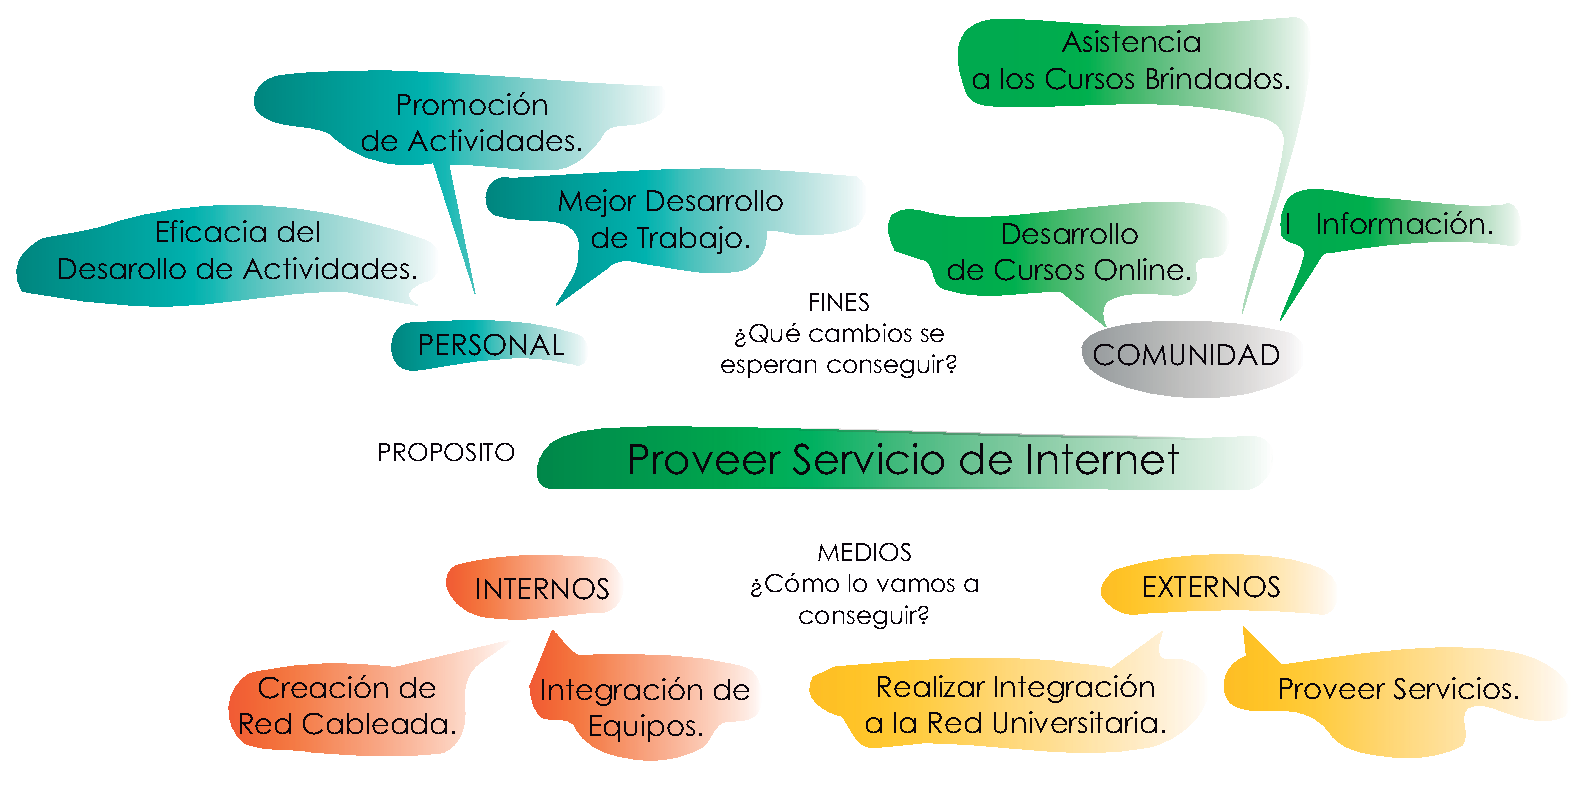
\includegraphics[width= 1 \linewidth]{ArbolDeObjetivos.eps}
    \caption{Árbol de objetivos}
    \label{fig:problem_tree}
\end{figure}

%%%%%%%%%%% METODOLGOÍA %%%%%%%%%%%%%%%%%%%%%%%%%%%%%%%%%%%%%%%

\chapter{Metodología}
El desarrollo del Proyecto de Servicio Comunitario, referido al diseño de un radioenlace entre el núcleo San Diego de la Dirección de Extensión y Servicio Comunitario y la Dirección de Medios Electrónicos y Telemática, ambos organismos adscritos a la Universidad de Carabobo, comprende; entre sus diversas partes, de un examen detallado de la descripción de la zona en la cual se implementará el mencionado proyecto, la identificación de los organismos gubernamentales que hacen vida en la zona, los recursos materiales y humanos con los que cuenta la comunidad y los organismos encargados de la implementación del diseño propuesto y una esquematización adecuada de las tareas que deben ser ejecutadas durante toda la evolución del proyecto de servicio comunitario. En ese sentido, el presente apartado desglozará cada uno de los puntos mencionados basándose en la información suministrada por el personal administrativo de DESCO San Diego, los vecinos de las comunidades adyacentes y valiéndose de la información  obtenida en el último censo oficial de población y vivienda, ejecutado por el Instituto Nacional de Estadística en el año 2011.

\section{Descripción de la zona de estudio}
El diseño del radioenlace, objeto último del proyecto de Servicio Comunitario, está destinado al núcleo San Diego de la Dirección de Extensión y Servicio Comunitario de la Universidad de Carabobo. Dicha entidad se ubica en el municipio San Diego del Estado Carabobo y es adyacente al \textbf{Conjunto Residencial \textit{El Tulipán}}. Un esquema de la ubicación relativa de la dirección con respecto a la Facultad de Ingeniería de la UC se muestra a continuación.

\begin{figure}[h]
	\centering
	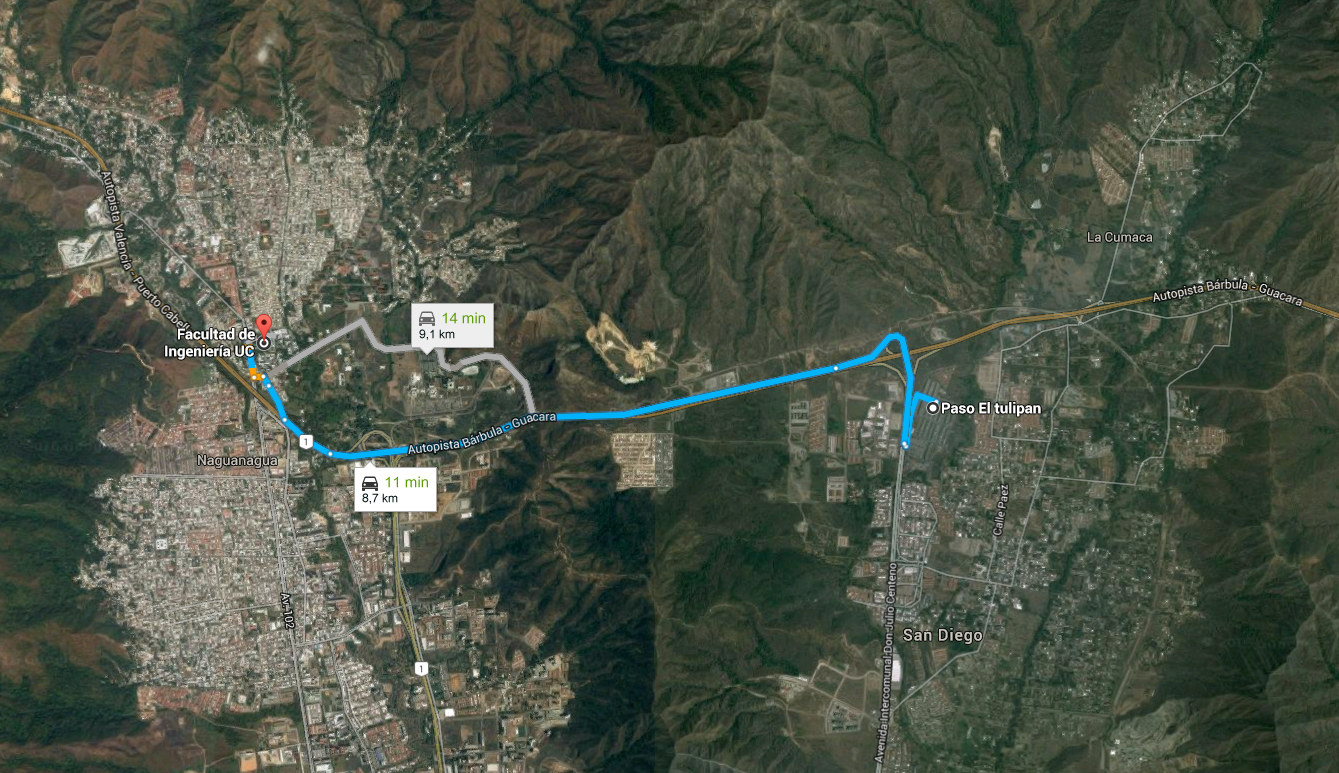
\includegraphics[width=0.5\textwidth]{fig1}
	\caption{Ubicación relativa de DESCO San Diego. \textit{Fuente: Google Maps 2016}}
\end{figure}

El Núcleo DESCO San Diego está constituido principalmente por 3 edificios, de los cuales 2 son los que se encuentran operativos, el ubicado en la posición central (Señalado en la figura \ref{f2}) es donde tienen lugar los cursos y actividades comunitarias planificadas mensualmente por la dirección, el edificio contiguo pertenece a la facultad de Odontología de la Universidad de Carabobo y en la actualidad, no se desarrolla ningún tipo de actividad en dicho recinto. Las \textbf{Coordenadas Geográficas} del Salón de Actividades Comunitarias son: $10^{\circ}16'22.0"N 67^{\circ}57'32.8"W$.

\begin{figure}[h]
	\centering
	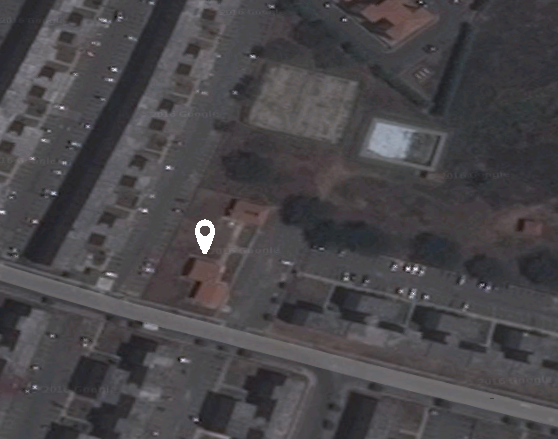
\includegraphics[width=0.5\textwidth]{fig2}
	\caption{Salón de Actividades Comunitarias de DESCO San Diego. \textit{Fuente: Google Maps 2016}}
	\label{f2}
\end{figure}
\subsection{Servicios Básicos Disponibles}
\begin{itemize}
	\item Servicio de electricidad suministrado por la Corporación Eléctrica Nacional (\textit{CORPOELEC}).
	\item Suministro de agua corriente por pozo profundo.
	\item Servicio de aseo urbano proporcionado por el Instituto Autónomo de Función, Mantenimiento y Conservación Urbana y Ambiental del Municipio San Diego (\textit{I. A. M FUMCOSANDI}).
\end{itemize}

\subsection{Características de la Población}

La Dirección de Extensión y Servicio Comunitario de la Universidad de Carabobo, a fin de ofrecer un servicio orientado a satisfacer las necesidades específicas de cada comunidad, se organiza en una serie de núcleos ubicados en cada uno de los municipios del estado carabobo; en consecuencia, la población potencialmente beneficiaria de las actividades y servicios ofrecidos por DESCO San Diego consta, de acuerdo a la información suministrada por \footnote{INE. XIV  Censo  Nacional  de  Población  y Vivienda. Ministerio del Poder Popular de Planificación , 2011.}, de 93.257 personas, integrantes de aproximadamente 25683 familias \footnote{Cabe destacar que el municipio San Diego alberga el 4.1 $\%$ del total poblacional del estado Carabobo.}, de los cuales 52.51 $\%$ son mujeres y 47.48 $\%$ hombres. De todos estos, el 73 $\%$ tiene una edad comprendida entre 15 a 64 años, seguidos por el grupo etario de menores de 15 años (21 $\%$) y por último, el de mayores de 63 años (5.9 $\%$). Si bien no se estima, de acuerdo a las estadísticas proporcionadas por el personal del núcleo, que el grueso de esta población participe simultáneamente en cada una de las actividades programadas por la dependencia, la oferta educativa y cultural propuesta por el núcleo está orientada a satisfacer las necesidades y gustos particulares de esta muestra poblacional, constituyéndose, de esta forma, en potenciales usuarios y usuarias. 

A nivel socio-económico, la mayor parte de la población se ubica en el estrato socio-económico III, denominado también \textit{Clase C} o \textit{Clase Media-Alta y Clase Media} seguidos por el estrato IV, (\textit{Clase D o \textit{Clase Media Baja - Pobreza Moderada}}).

\begin{table}[h]
	\centering
	\begin{tabular}{|c|c|}
		\hline
		\cellcolor{gray75} \textbf{Estrato Socioeconómico} & \cellcolor{gray75} \textbf{Total ($\%$)} \\ \hline
		Estrato I & 1.1 \\ \hline
		Estrato II  & 18.9 \\ \hline
		Estrato III & 50 \\ \hline
		Estrato IV & 28.9 \\ \hline
		Estrato V & 1.1 \\ \hline
	\end{tabular}
	\caption{Estratificación Socioeconómica en el municipio San Diego. \textit{Fuente: INE}}
	\label{tabla1}
\end{table}

\subsection{Sitios Relevantes adyacentes a la Zona de Estudio}
El Núcleo DESCO San Diego se encuentra rodeado por el Conjunto Residencial Los Tulipanes, a 58 metros en dirección noreste hay una cancha de fútbol rodeada por maleza, sin porterías ni gradas, a 380 metros en dirección suroeste está ubicado un módulo de la Policía Municipal de San Diego; resalta la ausencia de bodegas y supermercados a un radio de 500 metros del núcleo, lo cual puede dificultar la permanencia del personal administrativo, facilitadores y beneficiarios en el recinto por períodos prolongados.

\subsection{Beneficiarios del Proyecto de Servicio Comunitario}
De acuerdo a los datos obtenidos del órgano divulgativo de DESCO San Diego, la distribución del número de beneficiarios directos de los proyectos desarrollados por la dirección a lo largo del año corresponde a lo expuesto en la tabla \ref{tabla2}

\begin{table}[h]
	\centering
	\begin{tabular}{|c|c|}
		\hline
		\multicolumn{2}{|c|}{\cellcolor{gray75} \textbf{Beneficiarios Directos}}                  \\ \hline
		\multirow{2}{*}{\textbf{Trimestre}} & \textbf{Ejecutado}               \\ \cline{2-2} 
		& \textbf{Número de Beneficiarios} \\ \hline
		I                                   & 528                              \\ \hline
		II                                  & 718                              \\ \hline
		III                                 & 517                              \\ \hline
		IV                                  & 122                              \\ \hline
		\textbf{Total}                      & \textbf{1885}                    \\ \hline
	\end{tabular}
		\caption{Beneficiarios Directos DESCO. \textit{Fuente: Espacio DESCO San Diego}}
		\label{tabla2}
\end{table}
El total de beneficiarios directos del espacio DESCO San Diego se reparten, según su género, de acuerdo a lo expuesto en la tabla \ref{tabla3}

\begin{table}[h]
	\centering
	\begin{tabular}{|c|c|c|c|}
		\hline
		\multicolumn{4}{|c|}{\cellcolor{gray75} \textbf{Clasificación por Sexo}}                        \\ \hline
		\textbf{Trimestre} & \textbf{Masculino} & \textbf{Femenino} & \textbf{Total} \\ \hline
		I                  & 113                & 415               & 528            \\ \hline
		II                 & 229                & 489               & 718            \\ \hline
		III                & 158                & 359               & 517            \\ \hline
		IV                 & 58                 & 64                & 122            \\ \hline
		\textbf{Total}     & \textbf{558}       & \textbf{1327}     & \textbf{1885}  \\ \hline
	\end{tabular}
	\caption{Beneficiarios Directos DESCO San Diego: Clasificación por Sexo \textit{Fuente: Espacio DESCO San Diego}}
	\label{tabla3}
\end{table}
En cuanto a grupos etarios, la clasificación se desarrolla como lo muestra la tabla \ref{tabla3}.

\begin{table}[h]
	\centering
	\begin{tabular}{|c|c|c|}
		\hline
		\multicolumn{3}{|c|}{\cellcolor{gray75} \textbf{Grupos Etarios}}                     \\ \hline
		\textbf{Edades} & \textbf{Personas Atendidas} & \textbf{Posición} \\ \hline
		\textbf{3-8}    & 259                         & 2                 \\ \hline
		\textbf{9-14}   & 418                         & 1                 \\ \hline
		\textbf{15-20}  & 157                         & 5                 \\ \hline
		\textbf{21-26}  & 156                         & 6                 \\ \hline
		\textbf{27-32}  & 130                         & 7                 \\ \hline
		\textbf{33-38}  & 189                         & 3                 \\ \hline
		\textbf{39-44}  & 111                         & 9                 \\ \hline
		\textbf{45-50}  & 171                         & 4                 \\ \hline
		\textbf{51-56}  & 121                         & 8                 \\ \hline
		\textbf{57-62}  & 60                          & 10                \\ \hline
		\textbf{63-68}  & 111                         & 9                 \\ \hline
		\textbf{69-74}  & 2                           & 11                \\ \hline
		\textbf{Total}  & \multicolumn{2}{c|}{\textbf{1885}}              \\ \hline
	\end{tabular}
	\caption{Beneficiarios Directos DESCO San Diego: Grupos Etarios \textit{Fuente: Espacio DESCO San Diego}}
	\label{tabla3}
\end{table}
Partiendo de los datos expresados en el apartado, la mayoría de los beneficiarios del espacio DESCO San Diego son mujeres de entre 9 a 14 años que asisten, principalmente, durante el segundo trimestre del año.\\
De acuerdo a las indicaciones de la Licenciada Fanny Barrios, coordinadora del Núcleo San Diego de DESCO, los beneficiados indirectos de las actividades y proyectos desarrollados por el organismo son los habitantes del municipio San Diego del Estado Carabobo.

\section{Situación organizativa}
\subsection{DESCO San Diego}
La coordinación del Espacio San Diego de la Dirección de Extensión y Servicio Comunitario de la Universidad de Carabobo está a cargo de:

\begin{itemize}
	\item \textbf{Nombre:} Licenciada Fanny Barrios.
	\item \textbf{C.I.:} V - 13.497.625.
	\item \textbf{Teléfono de Contacto:} +58 416 294.14.52.
	\item \textbf{Correo Electrónico:} espaciosandiego@gmail.com.
\end{itemize}

\section{Recursos disponibles}

\subsection{Humanos}
Los recursos humanos de DESCO San Diego están constituidos por sus autoridades y coordinadores, quienes son los encargados de planificar y ejecutar la mayoría de las actividades que tienen lugar en el núcleo; del mismo modo, miembros de la Policía Municipal de San Diego, Cuerpo de Protección Civil y personal de la Cruz Roja, se ofrecen esporádicamente para dictar cursos de Seguridad Ciudadana, Atención de Desastres y Primeros Auxilios; por último, los estudiantes de todas las facultades de la Universidad de Carabobo tienen en DESCO un espacio para desarrollar sus proyectos de Servicio Comunitario, dentro de sus respectivos ámbitos de experticia, formando parte así del recurso humano de la dependencia universitaria. En lo que respecta a los recursos humanos disponibles para la implementación del diseño propuesto, se cuenta por el personal de la Dirección de Medios Electrónicos y Telemática de la Universidad de Carabobo, quienes poseen la experticia técnica y la experiencia de campo necesarias para la ejecución de las diferentes etapas comprendidas por el proyecto.

\subsection{Materiales}
DESCO San Diego ofrece un recinto amplio y limpio para el desarrollo de actividades de distinta índole, cuenta con una dotación básica de mobiliario (Sillas, Mesas y Escritorios) para facilitar las tareas de coordinadores y participantes; sin embargo, son los beneficiarios quienes deben procurarse para sí los materiales necesarios para la realización de cada actividad específica, la coordinación informa oportunamente a los usuarios sobre los recursos materiales que se necesitarán en cada actividad.
El núcleo DESCO San Diego proporciona un área despejada lo suficientemente amplia como para garantizar la factibilidad de la instalación de un poste sobre el cual podrán instalarse las estructuras radiantes requeridas para la implementación del radioenlace propuesto.

\subsection{Económicos}
 DESCO San Diego no cobra por la realización de sus actividades ni cuenta con una forma de financiación adicional a los recursos asignados a través de la partida presupuestaria de la universidad, esta última constituye la instancia que proporcioná la eventual financiación para la construcción de las estructuras y adquisión de equipos necesarios para la materialización del diseño propuesto.
 
 \newpage
\section{Diagrama de Gantt}
 El diagrama de Gantt es un tipo de esquematización de un conjunto de tareas que deben ejecutarse en un lapso previsto para la consecución de un fin determinado, en el mismo están implícitas las relaciones entre cada una de las tareas; sin embargo, las mismas pueden llegar a ser indicadas como forma de hacer énfasis en el orden que un equipo de trabajo debe seguir.\\

 \begin{figure}[H]
 	\centering
 	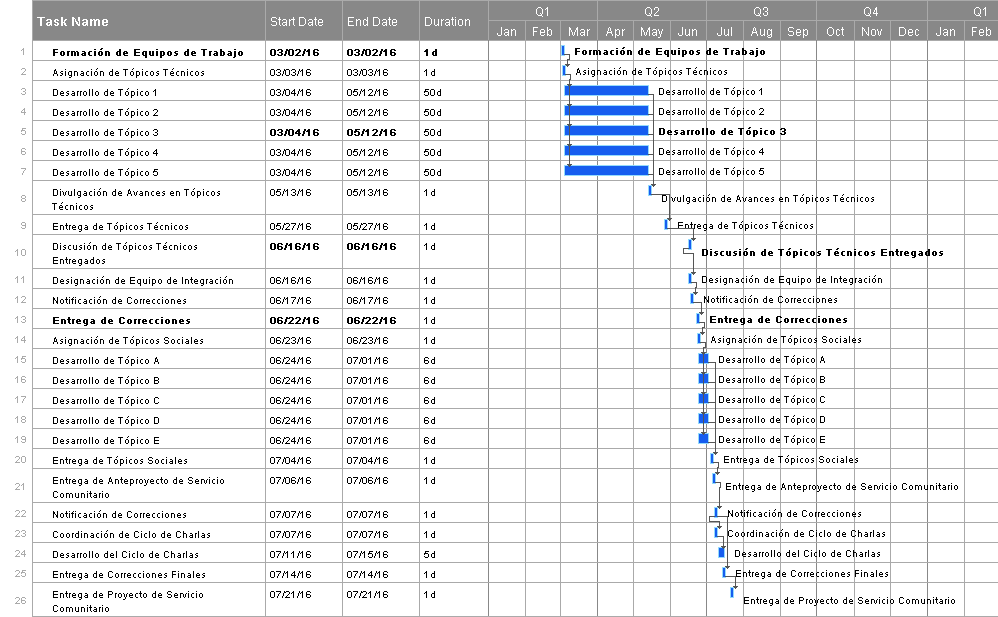
\includegraphics[width=1\textwidth, height=17cm, angle=270]{fig3}
 	\caption{Diagrama de Gantt. Periodo de Actividades: 03-03-2016 al 21-07-2016. \textit{Fuente: Smartsheets}}
 \end{figure}
 
%%%%%%%%%%%% DESCRIPCIÓN %%%%%%%%%%%%%%%%%%%%%%%%%%%%%%%%%%%%%%%%%%5
\chapter{Descripción de los servicios del\\ proyecto}
Desde el momento que se inició dicho proyecto, se observó que la Dirección de Extensión y Servicio Comunitario (DESCO) posee una situación de déficit en cuanto a los servicios de comunicación y computadoras.

Es por ello que los estudiantes de Ingeniería de Telecomunicaciones, aportan una solución robusta y efectiva para la implementación del servicio a internet mediante la aplicación de un enlace de microondas que proporcionará no solo el acceso a internet, sino que a futuro se podrá orientar a la comunidad sobre las técnicas y el uso adecuado de éste servicio, agregándole otra cualidad a la institución lo cual se traduce en educación para no sólo las comunidades cercanas sino para ciudadanos de otras localidades que deseen aprender.

En cuanto a los recursos necesario para llevar a cabo la realización del proyecto, se requiere, principalmente, personal capaz de ejecutar las tareas previstas para cumplir los objetivos del proyecto. También materiales como tubos PVC, conexiones PVC, además de cable UTP cat5 y conectores RJ-45 serán necesarios para la canalización correspondiente. Para la gestión de conexiones de la red dentro de la institución, serán necesarios equipos como switches y routers los cuales brindaran acceso a la red a los usuarios, estos equipos necesitaran de un soporte o un rack y de un UPS para su correcta operación.

Para la ubicación de la antena, se debe disponer del soporte necesario para el equipo transmisor que compone el radio enlace en DESCO, así como también de espacio suficiente dentro de la posición calculada para el radio enlace, para la instalación de dicho soporte.
Del lado del cerro La Cruz ya se encuentra la infraestructura necesaria para implementar el radio enlace, por lo que solo haría falta la instalación de la antena y el cableado correspondiente.
(Acotar que en el apéndice se encuentra cada dato de este servicio)


%%%%%%%%%%%% RESULTADOS  %%%%%%%%%%%%%%%%%%%%%%%%%%%%%%%%%%%%%%%%%%5
\chapter{Resultados obtenidos}
Mediante el software de simulación RadioMobile fue posible asegurar la línea de vista entre ambas antenas, además se obtuvo una visión más general acerca de la cobertura de la misma.

\begin{figure}[h]
    \centering
    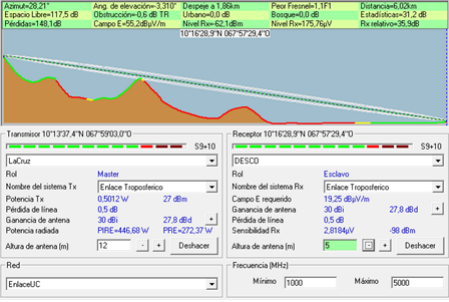
\includegraphics[width=0.55\linewidth]{rm.png}
    \caption{Parámetros del Radioenlace DESCO-Cerro la Cruz. Radio Mobile}
    \label{fig:rm}
\end{figure}

En la figura se puede constatar el nivel de señal promedio y su umbral de recepción, con esto es posible verificar que el enlace tiene la suficiente potencia para establecer la conexión sin inconvenientes 

\begin{itemize}
\item Intensidad de campo: $55, 2dB\mu/m$
\item Capacidad del Enlace: $230.38 Mbps$
\item Nivel Rx: $-62,1dBm$
\item Despeje: $1, 86km$
\item Pérdidas: $148,1dB$
\end{itemize}

Finalmente, en los apendices se muestra el mapa de cobertura del enlace, garantizando que la DESCO-San Diego está ubicada en una zona óptima para la recepción. Con todos estos datos es posible asegurar que siguiendo las indicaciones de instalación aquí descritas el radioenlace funcionará de forma plena y satisfactoria.


%%%%%%%%%%%% EJECUCIÓN  %%%%%%%%%%%%%%%%%%%%%%%%%%%%%%%%%%%%%%%%%%5
\chapter{Ejecución y seguimiento}
El  actual proyecto de servicio comunitario se compone en dos fases, ambas enfocadas en la etapa de diseño, la primera de ellas consiste en la realización de un enlace de microondas entre el módulo DESCO ubicado en la urbanización Tulipan del Municipio San Diego enlazado con  la antena principal que brinda servicio de datos s a la Universidad De Carabobo ubicada en Cerro La Cruz. En la fase final del proyecto, una vez garantizada la recepción de la señal (etapa inicial) se realiza el diseño del cableado estructurado, la evaluación de los equipos necesarios para la distribución de varios puntos de datos a lo largo del recinto de manera que se garantice la  disposición del servicio de internet en todo el recinto. 

Para el diseño del enlace de microondas se realizó una  simulacion con el software RadioMobile, el cual mendiante datos de elevación construye la gráfica del perfil del terreno, además de calcular el modelo de propagación que surge en terrenos irregulares, para realizar todo esto es necesario el ingreso de paramtros como la ubicación y la altura de ambas antenas (Emisora Tx y Receptora Rx), frecuencias de operación, ganancias Tx y RX, sensibilidad en la antena receptora, patrones de radiacion, entre otros que se especifican en los anexos del presente trabajo.

Para la etapa final, en el diseño del cableado estructurado una vez conocida la cantidad de puntos de datos requeridos en la sede, se precedió a seleccionar el switch y los routers inalámbricos acordes a las necesidades, luego mediante el uso del software PacketTracer se realizo una pequeña simulacion en la que aprecia la topología y los dispositivos mencionados.

Aunado a la etapa de simulación  se acudió tanto a Cerro La cruz como a la sede DESCO en tulipán para evaluar las instalaciones y verificar los resultados obtenidos, enfocándonos principalmente en en la línea de vista del enlace, la ubicación de los puntos de red, el cableado principal de la antena receptora al switch, la ubicación del rack y las tuberías para el tendido del cable de red.
Todos los parámetros tecnicos, especificaciones y equipos necesarios para la realización del proyecto son como se ha dicho anteriormente indicados en los anexos.

\textbf{Fases cumplidas}: Todo lo referente a la etapa de evaluación y factibilidad de un proyecto de ingeniería, abarcando la etapa de diseño y estimación de costos.

\textbf{Fases por cumplir}: La impementacion, queda por realizar la instalación de los equipos por parte de la dirección de planta física de la Universidad De Carabobo una vez que sean aprobados los recursos económicos para concretar con éxito el proyecto


%%%%%%%%%%%% CONCLUSIONES  %%%%%%%%%%%%%%%%%%%%%%%%%%%%%%%%%%%%%%%%%%5
\chapter{Conclusiones} 
Hoy en día aquellas comunidades de la Desco que no tenían una ayuda, que eran totalmente desasistidas están siendo atendidas por su máxima labor de organizarse como comunidad y elaborar proyectos para una mejora en su sector, así como también tienen la oportunidad de recibir a grupos de estudiantes que van con el objetivo de cumplir 120 horas de servicio comunitario en pro de una mejor calidad de vida ya que en esta se realiza diversas actividades donde la comunidad de la Desco son nuestro objetivo.

Como primer objetivos se hizo una visita a la Desco en la cual se evaluó como se haría una propuesta para ver cómo se haría la instalación de la antena y de la red interna, luego se hicieron los cálculos correspondiente para saber dónde establecerían el lugar de antenas y luego una etapa del cálculo del radio enlace en el cual por medio de software se hizo el estudio en el cual fueron factible la ubicación de la antena en la Desco en cuanto a los cálculos. Luego se hizo un estudio para la red interna en el cual se hizo una lista de equipos necesario para que funcionara la red interna luego también se hicieron planos de la instalación en el cual en el cual se plantearía de cómo será la canalización de la red interna.



%%%%%%%%%%%% RECOMENDACIONES  %%%%%%%%%%%%%%%%%%%%%%%%%%%%%%%%%%%%%%%%%%
\chapter{Recomendaciones} 
\begin{enumerate}
\item Este organismo ubicado en los tulipanes debería contar con una página web o página de servicios donde su pudiese acceder a las diversas actividades que se realizan allí con mayor facilidad para el público en general
\item Conseguir computadoras para poder realizar diversos cursos o talleres orientados hacia las comunicaciones, también para brindar servicios aquellos niños y jóvenes de la comunidad que por diversos motivos no tengan internet o equipos en sus casas con el fin de investigaciones.
\item Para que la comunidad consiga aprovechar al máximo dicho trabajo es importante que se lleven a cabo charlas explicativas sobre el servicio a ofrecer y cómo pueden ellos aprovechar esta herramienta para el desarrollo del emprendimiento por la web o emprendimiento 2.0 que fomente la creación de negocios o pequeñas empresas que contribuyan a la sustentabilidad de la comunidad.
\end{enumerate}


%%%%%%%%%%%%% MEMORIA FOTOGRÁFICA %%%%%%%%%%%%%%%%%%%%%%%%%%%%%%%%%%%%%%%

\chapter{Memoria fotográfica}

\begin{figure}[ht]
    \centering
    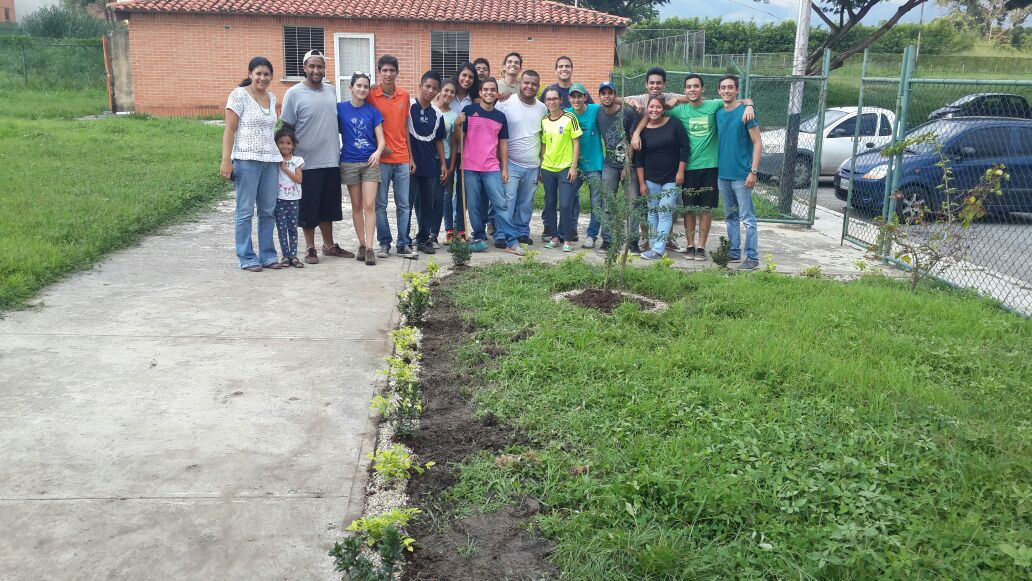
\includegraphics[width=0.76\linewidth]{1.jpg}
    \caption{Proyecto servicio comunitario DESCO-San Diego \#1}
    \label{fig:1}
\end{figure}

%\begin{figure}[ht]
%   \centering
%   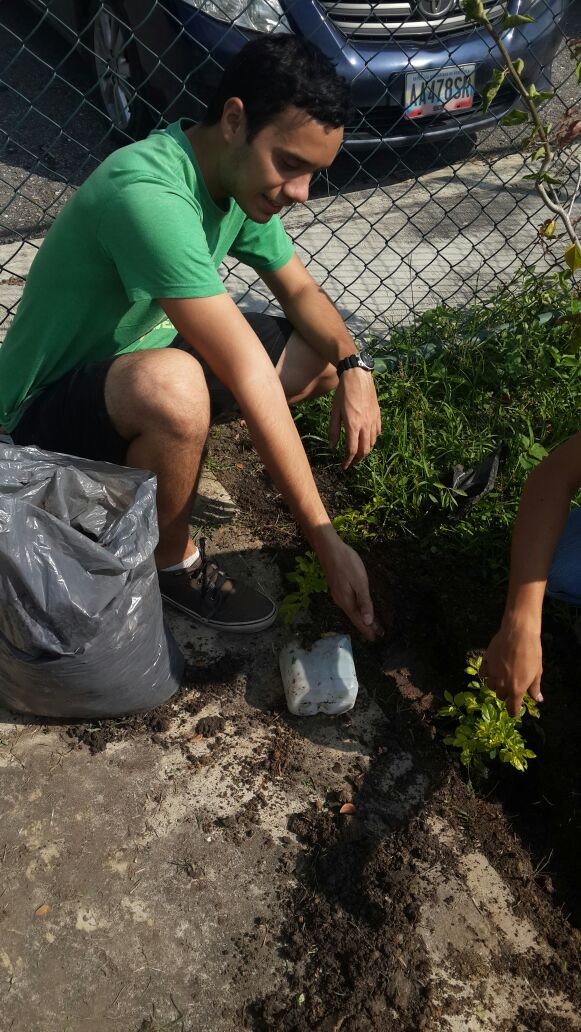
\includegraphics[width=0.4\linewidth]{2.jpg}
%   \caption{Proyecto servicio comunitario DESCO-San Diego \#2}
%   \label{fig:2}
%\end{figure}

%\begin{figure}[h]
%    \centering
%    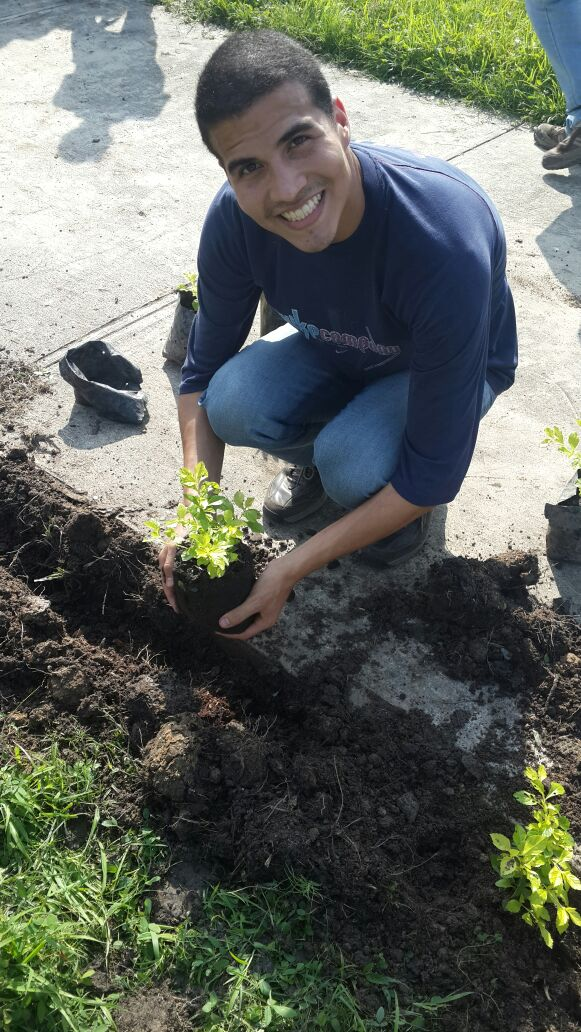
\includegraphics[width=1\linewidth]{3.jpg}
%    \caption{Proyecto servicio comunitario DESCO-San Diego \#3}
%    \label{fig:3}
%\end{figure}

\begin{figure}[h]
    \centering
    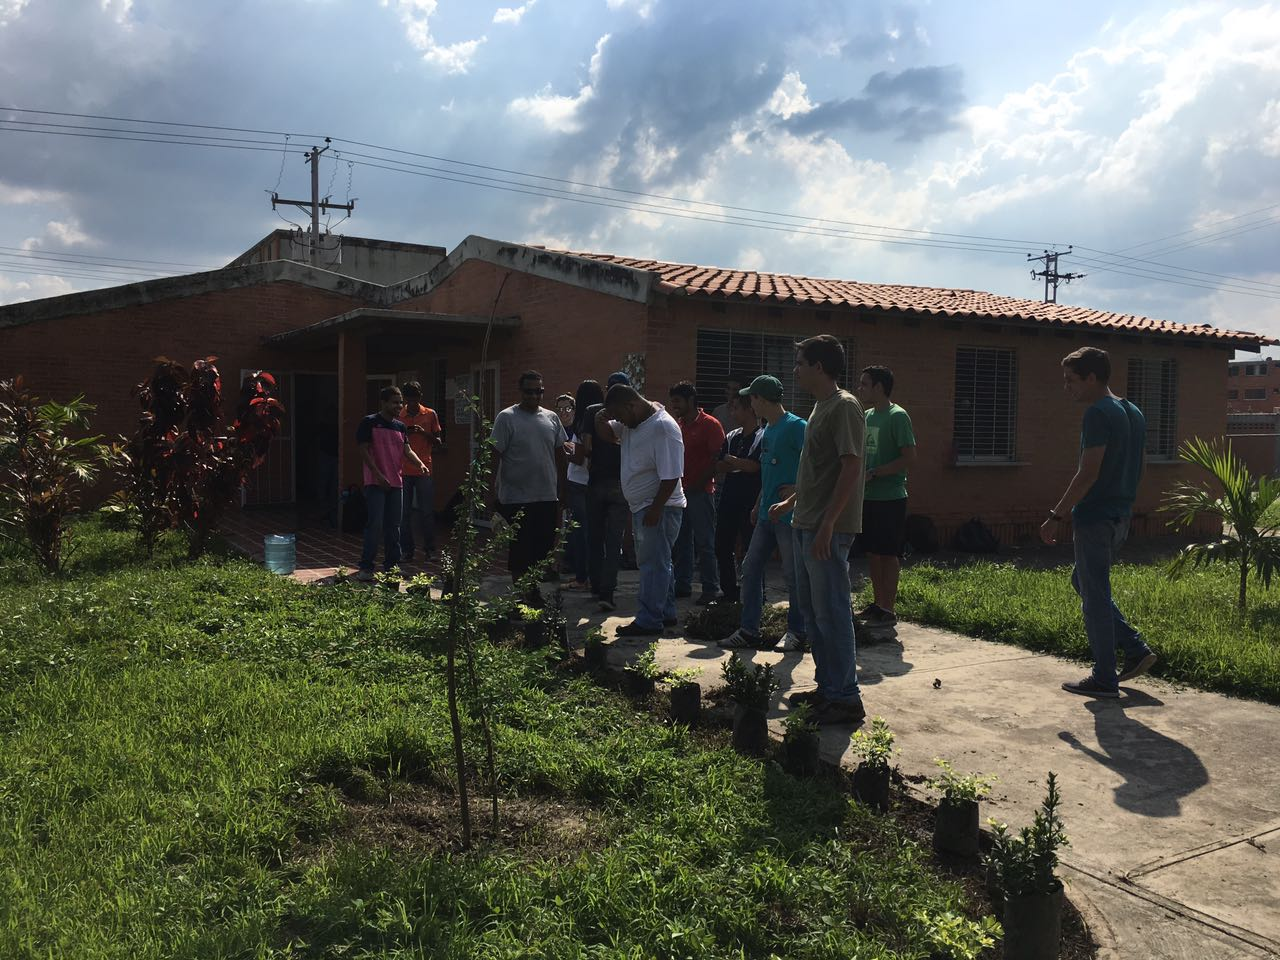
\includegraphics[width=0.76\linewidth]{4.jpg}
    \caption{Proyecto servicio comunitario DESCO-San Diego \#2}
    \label{fig:4}
\end{figure}

\begin{figure}[h]
    \centering
    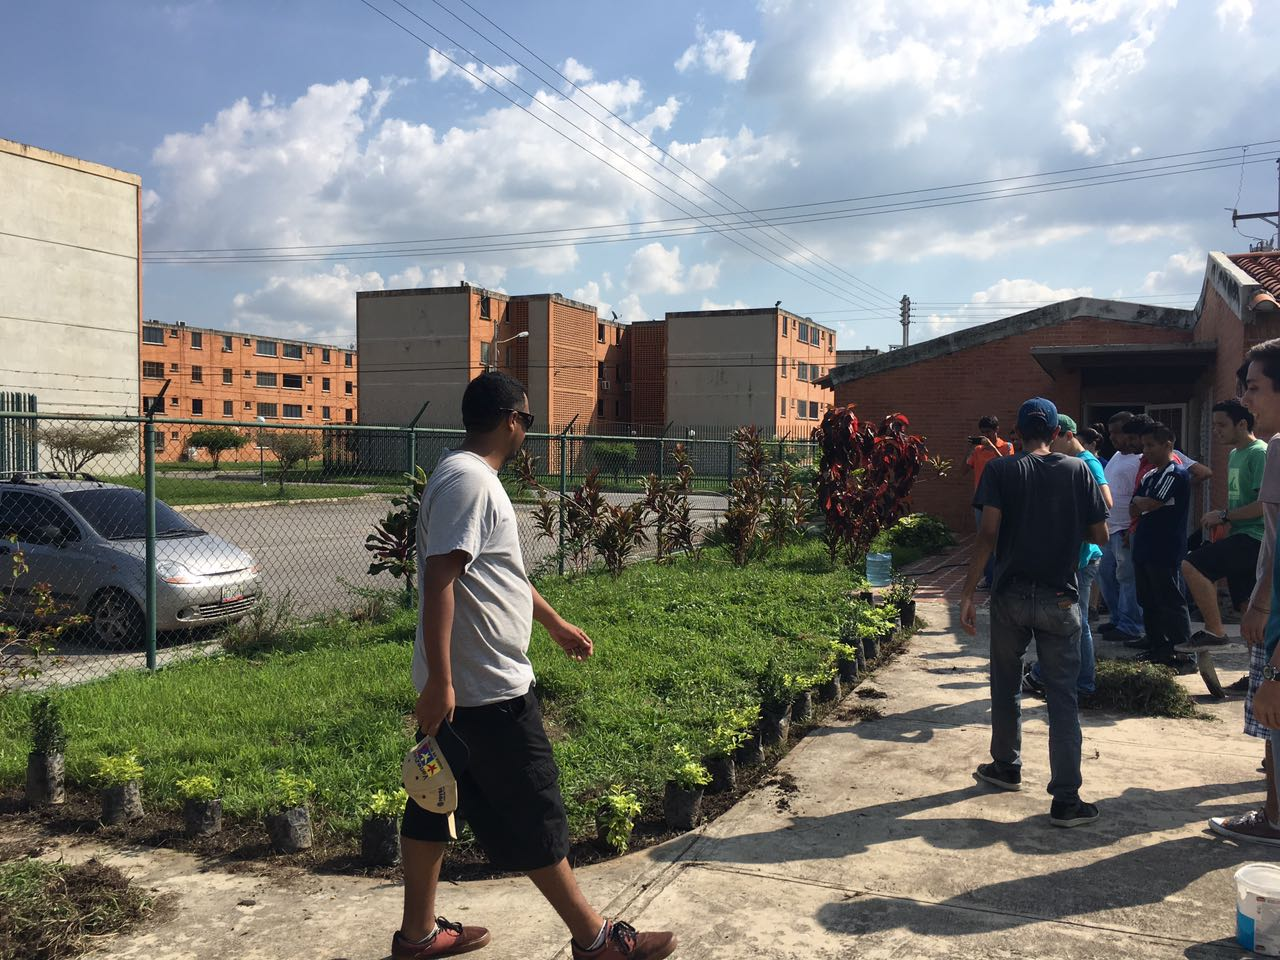
\includegraphics[width=1\linewidth]{5.jpg}
    \caption{Proyecto servicio comunitario DESCO-San Diego \#3}
    \label{fig:5}
\end{figure}

\begin{figure}[h]
    \centering
    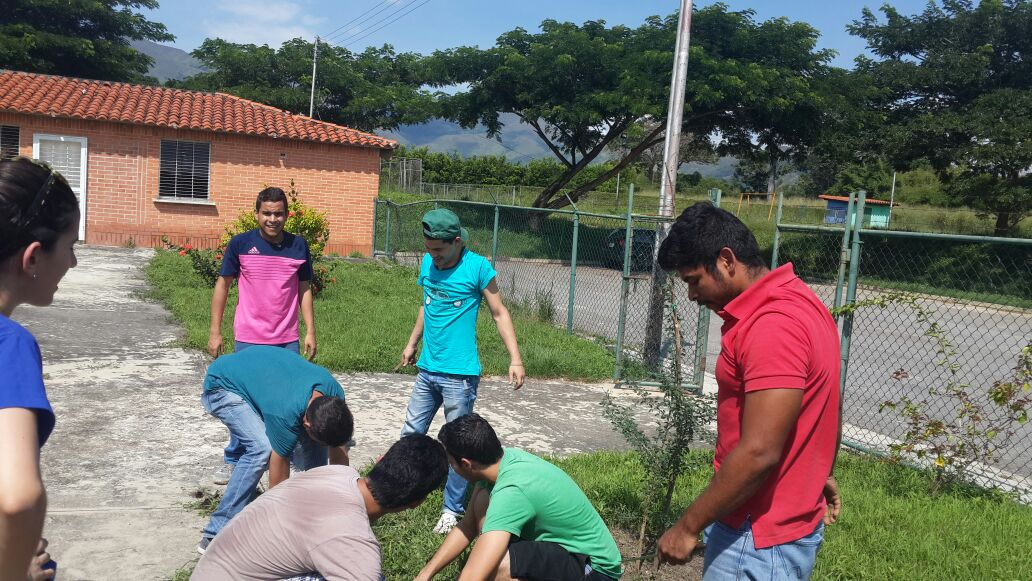
\includegraphics[width=1\linewidth]{6.jpg}
    \caption{Proyecto servicio comunitario DESCO-San Diego \#4}
    \label{fig:6}
\end{figure}

\begin{figure}[h]
    \centering
    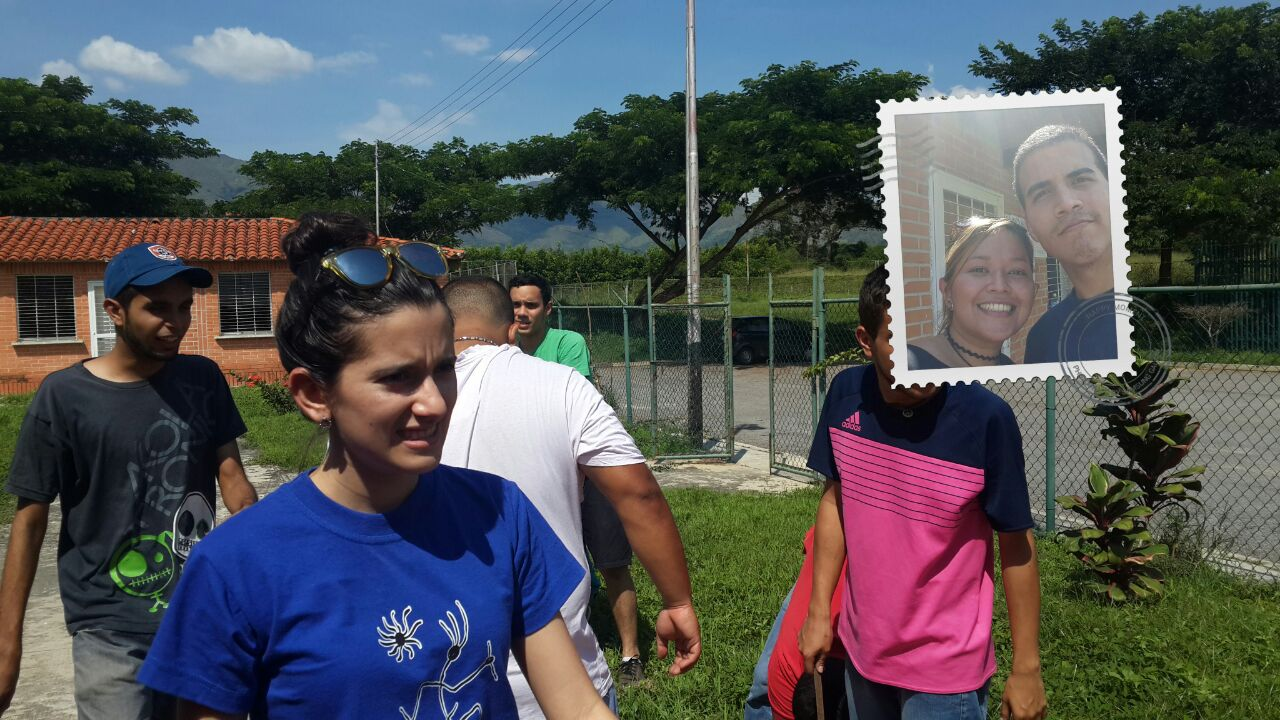
\includegraphics[width=1\linewidth]{7.jpg}
    \caption{Proyecto servicio comunitario DESCO-San Diego \#5}
    \label{fig:7}
\end{figure}

\begin{figure}[h]
    \centering
    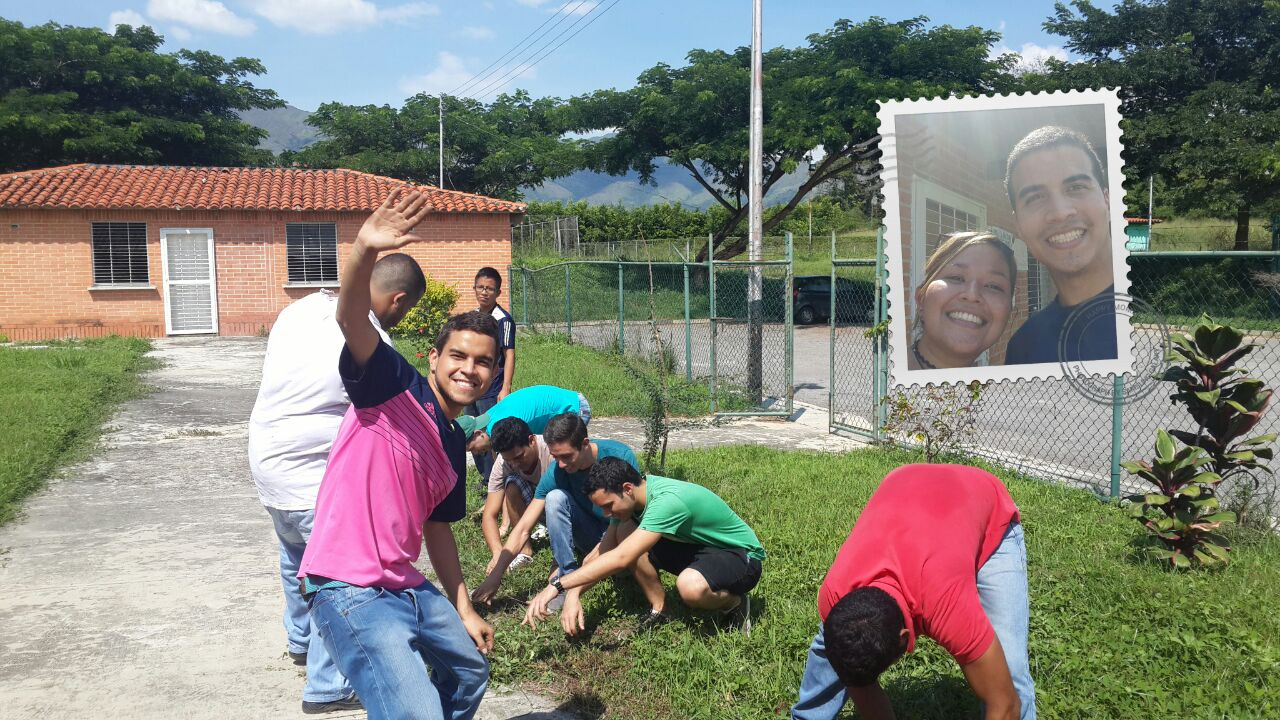
\includegraphics[width=1\linewidth]{8.jpg}
    \caption{Proyecto servicio comunitario DESCO-San Diego \#6}
    \label{fig:8}
\end{figure}

%\begin{figure}[h]
%    \centering
%    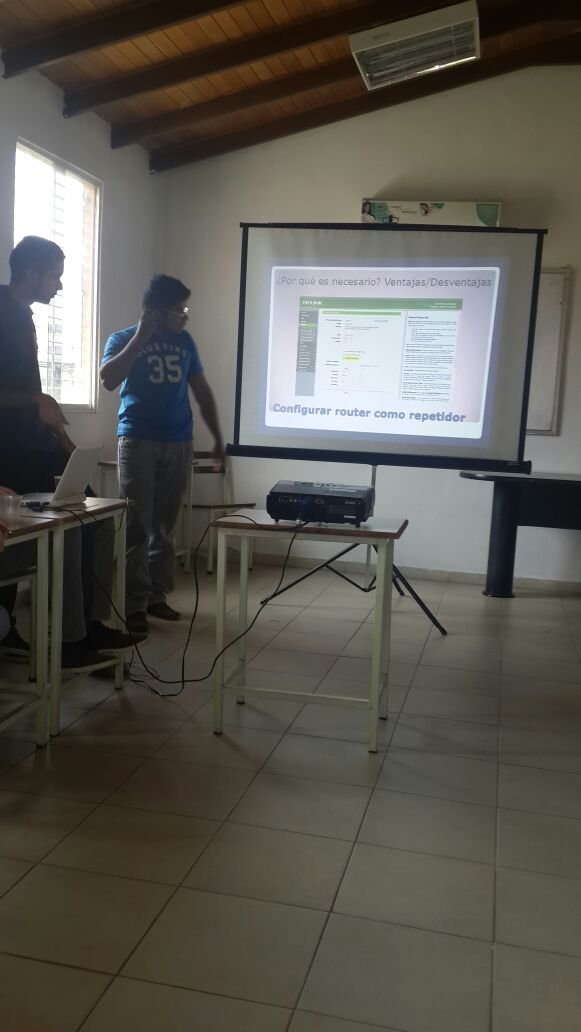
\includegraphics[width=1\linewidth]{9.jpg}
%    \caption{Proyecto servicio comunitario DESCO-San Diego \#7}
%    \label{fig:9}
%\end{figure}

\begin{figure}[h]
    \centering
    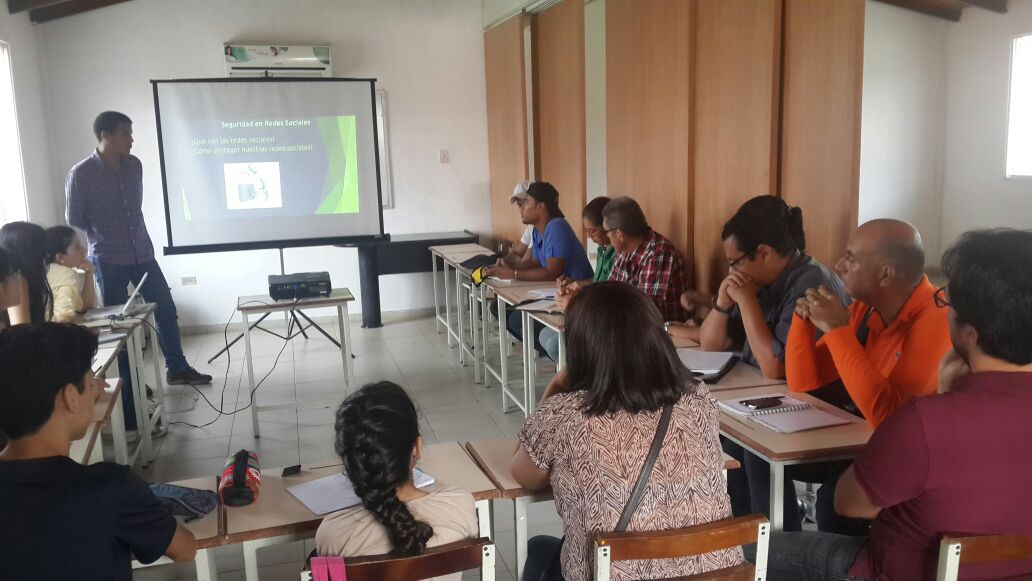
\includegraphics[width=1\linewidth]{10.jpg}
    \caption{Proyecto servicio comunitario DESCO-San Diego \#7}
    \label{fig:10}
\end{figure}

\begin{figure}[h]
    \centering
    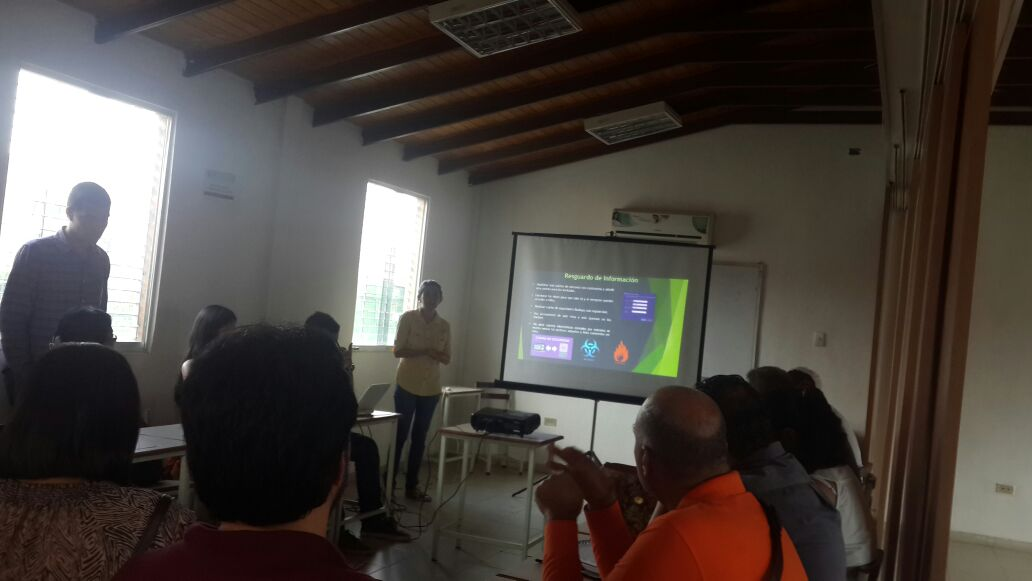
\includegraphics[width=1\linewidth]{11.jpg}
    \caption{Proyecto servicio comunitario DESCO-San Diego \#8}
    \label{fig:11}
\end{figure}

\begin{figure}[h]
    \centering
    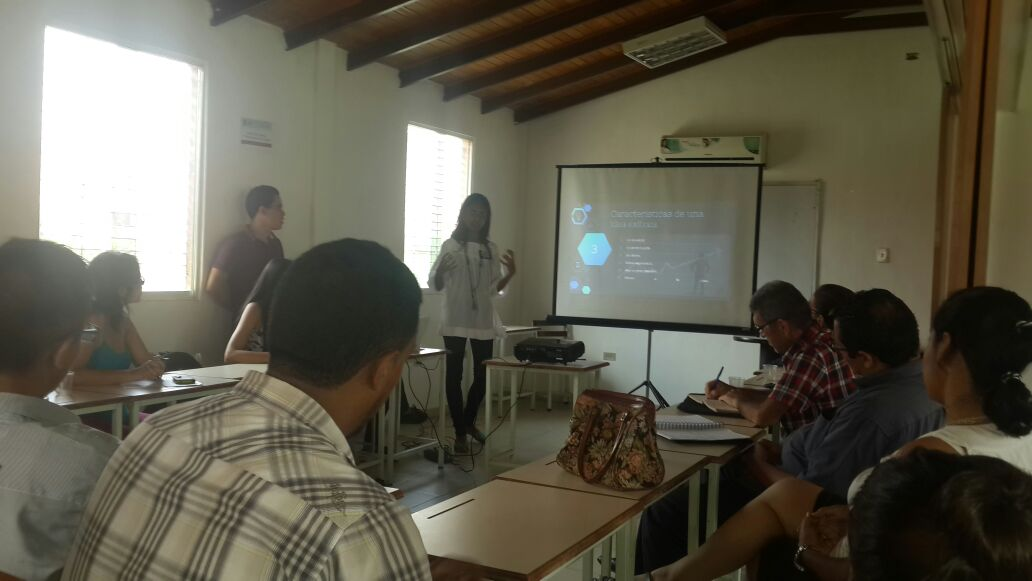
\includegraphics[width=1\linewidth]{12.jpg}
    \caption{Proyecto servicio comunitario DESCO-San Diego \#9}
    \label{fig:12}
\end{figure}

%\begin{figure}[h]
%    \centering
%    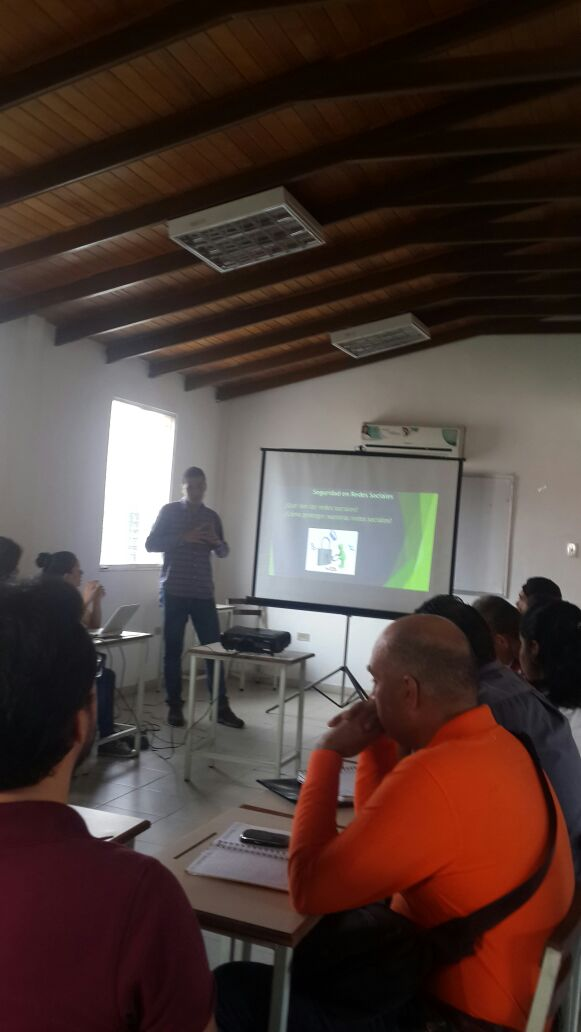
\includegraphics[width=1\linewidth]{13.jpg}
%    \caption{Proyecto servicio comunitario DESCO-San Diego \#13}
%    \label{fig:13}
%\end{figure}

\begin{figure}[h]
    \centering
    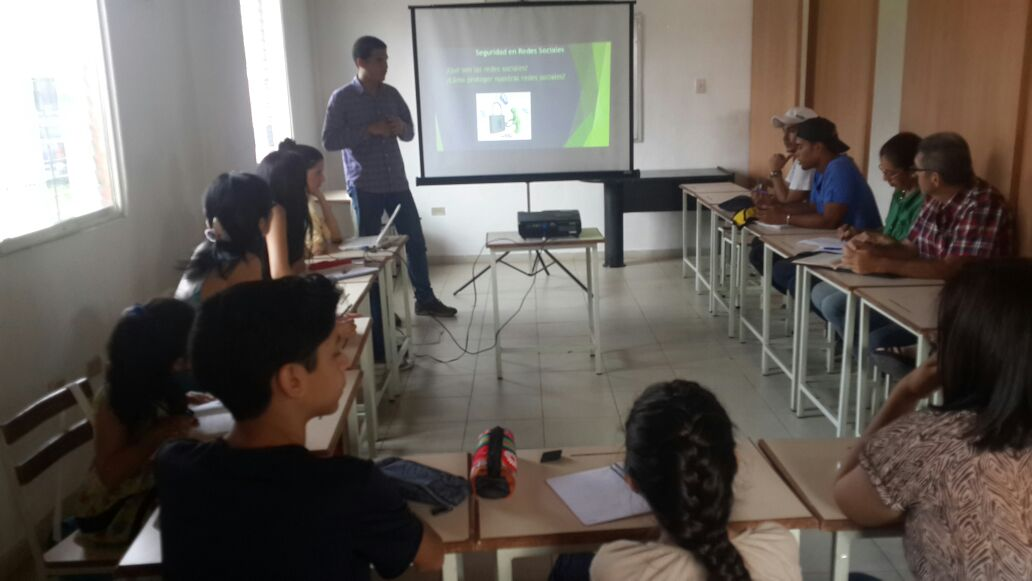
\includegraphics[width=1\linewidth]{14.jpg}
    \caption{Proyecto servicio comunitario DESCO-San Diego \#10}
    \label{fig:14}
\end{figure}

\begin{figure}[h]
    \centering
    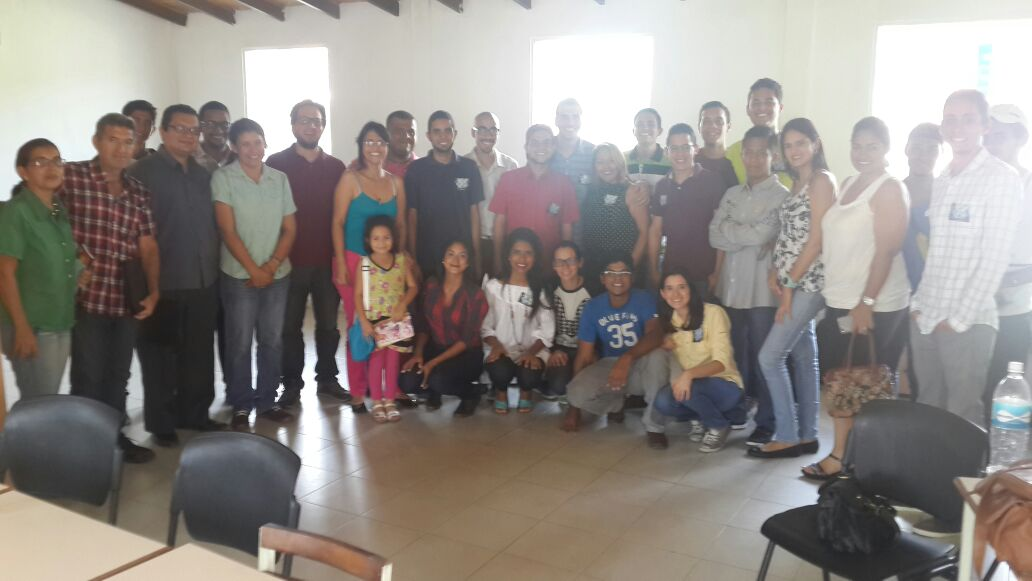
\includegraphics[width=1\linewidth]{n.jpg}
    \caption{Proyecto servicio comunitario DESCO-San Diego \#11}
    \label{fig:15}\end{figure}
%%%%%%%%%%% APÉNDICES %%%%%%%%%%%%%%%%%%%%%%%%%%%%%%%%%%%%%%%%
\appendix
\clearpage 
\addappheadtotoc
\appendixpage


\chapter{Descripción del radioenlace}
A continuación se comentaran los parámetros técnicos necesarios para el calculo de cobertura del radioenlace.

\section{Ubicación geográfica de las antenas}
Con ayuda del software Google Earth se determinaron las coordenadas geográficas de
la antena transmisora y receptora, las cuales son:

\noindent \textbf{Antena receptora}: Latitud: $10^{o}16'28,9''$ N. Longitud: $67^{o}57'29,4''$ O.\\
\noindent \textbf{Antena transmisora}: Latitud: $10^{o}13'37,35''$ N. Longitud: $67^{o}59'2,98''$ O.

La antena transmisora se ubica en la elevación topográfica denominada Cerro La Cruz tal como se muestra en la Fig. \ref{fig:ubiq}
\begin{figure}[h]
    \centering
    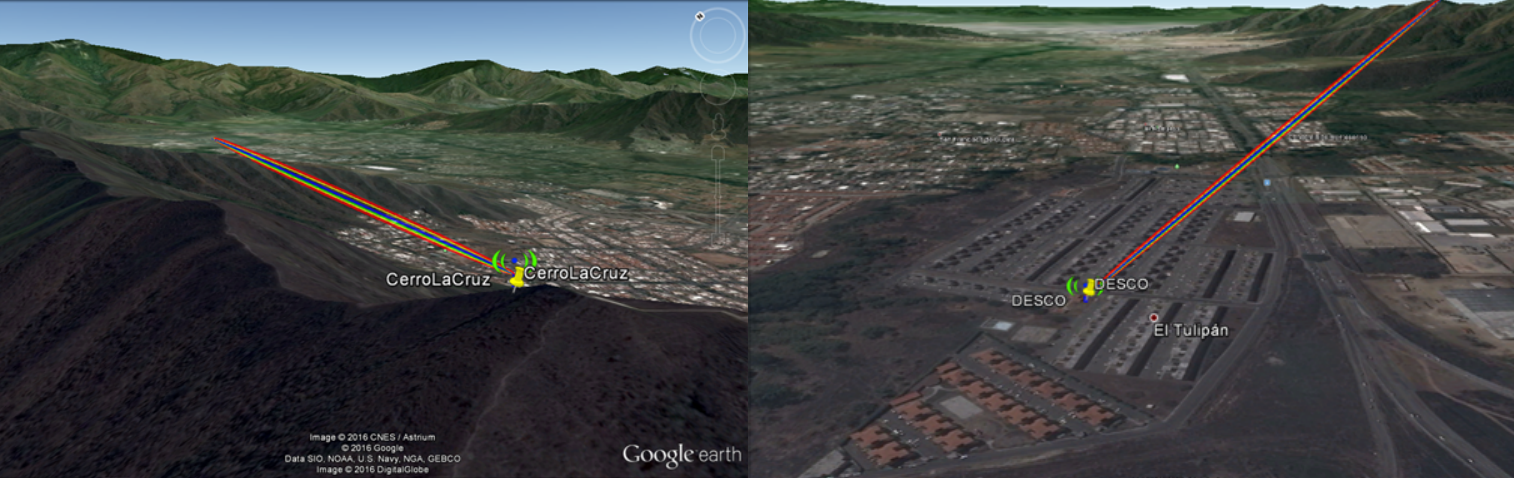
\includegraphics[width=1\linewidth]{ubiq.png}
    \caption{\textbf{Izq}. Línea de vista desde Cerro la Cruz hasta DESCO- San               Diego\\
            \textbf{Der}. Línea de vista desde  DESCO-San Diego hasta Cero la Cruz. Google Earth}
    \label{fig:ubiq}
\end{figure}

\section{Distancia entre Cerro la Cruz-DESCO }
\label{chap:radio}
Empleando el método autorizado para calcular distancias entre dos puntos por la FCC (Federal Comunications Comision) se tiene que:

\begin{equation}
    d(km) = \sqrt{(dlat \cdot \Delta lat)^{2} + (dlon \cdot \Delta lon)^{2}}
\end{equation}

Siendo $\Delta lat = Lat1 - Lat2$, $\Delta lon = Lon1 - Lon2$. La distancia de separación entre ambas antenas resulta ser: \textbf{$d = 5,987 km$}. Además para que ambas antenas se encuentre en línea de vista necesitan la siguiente orientación: 

Antena DESCO: Azimut  $208,25^{o}$, Elevación: $3,26^{o}$. \\
Antena Cerro-La Cruz: Azimut  $28,25^{o}$, Elevación: $-3,310^{o}$.

\section{Datos de la antena transmisora}

\begin{table}[ht]
\centering
 \begin{tabular}{|c|c|}
	\hline \cellcolor{gray75} Antena  & \cellcolor{gray75} airMAX AM-VG5-TI \\ 
	\hline Ubicación & Cerro la Cruz  \\ 
	\hline Altura sobre el suelo & $12m$ \\ 
	\hline Ganancia & $19dBi$\\ 
	\hline Potencia & $27 dBm$\\
	\hline Frecuencia de operación & $5,4 GHz$\\
	\hline 
\end{tabular}
\caption{Parámetros básicos de la antena transmisora}
\label{tab:AntC}
\end{table}

\subsection{Patrón de radiación de la antena}
\begin{figure}[h]
    \centering
    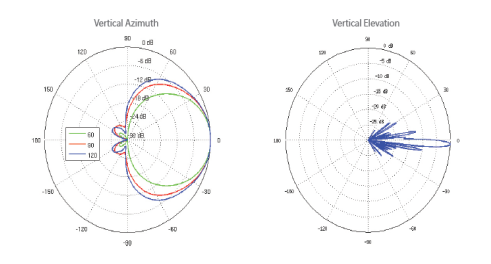
\includegraphics[width=1\linewidth]{antC.png}
    \caption{\textbf{Izq}. Azimuth .\textbf{Der}. Elevación. Manual de Ubiquti}
    \label{fig:antc}
\end{figure}
\newpage
\section{Datos de la antena receptora}
\begin{table}[ht]
\centering
 \begin{tabular}{|c|c|}
	\hline \cellcolor{gray75} Antena  & \cellcolor{gray75} NanoBridge NB-5G25 \\ 
	\hline Ubicación & DESCO-San Diego  \\ 
	\hline Altura sobre el suelo & $30m$ \\ 
	\hline Ganancia & $75dBi$\\ 
	\hline Sensibilidad & $-75 dBm$\\
	\hline Frecuencia de operación & $5,4 GHz$\\
	\hline 
\end{tabular}
\caption{Parámetros básicos de la antena receptora}
\label{tab:AntD}
\end{table}

\subsection{Patrón de radiación de la antena}
\begin{figure}[h]
    \centering
    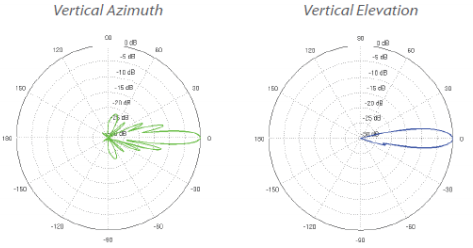
\includegraphics[width=1\linewidth]{antD.png}
    \caption{\textbf{Izq}. Azimuth .\textbf{Der}. Elevación. Manual de Ubiquti}
    \label{fig:antd}
\end{figure}

\section{Simulación en Radio mobile} 

Mediante el software de simulación Radio mobile fue posible asegurar la línea de vista entre ambas antenas, además se obtuvo una visión más general acerca de la cobertura de la misma. 

En la Fig. \ref{fig:rm}, se puede constatar el nivel de señal promedio y su
umbral de recepción, con esto es posible verificar que el enlace tiene la suficiente potencia para establecer la conexión sin inconvenientes.
\newpage

\begin{figure}[h]
    \centering
    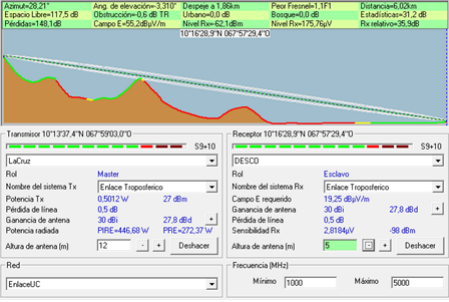
\includegraphics[width=0.55\linewidth]{rm.png}
    \caption{Parámetros del Radioenlace DESCO-Cerro la Cruz. Radio Mobile}
    \label{fig:rm}
\end{figure}

Los parámetros más importantes del radioenlace, calculados en la aplicación, pueden ser vistos en la siguiente tabla:

\begin{table}[ht]
\centering
 \begin{tabular}{|c|c|}
	\hline \cellcolor{gray75} Parámetro  & \cellcolor{gray75} Valor \\ 
	\hline Intensidad de campo & $55,2 dB\mu / m$  \\ 
	\hline Nivel Rx & $-62.1 dBm$ \\ 
	\hline despeje & $1,86 km$\\ 
	\hline Pérdidas& $148,1 dB$\\
	\hline 
\end{tabular}
\caption{Parámetros referentes a la calidad de la señal. Radio mobile}
\label{tab:sig}
\end{table}

Finalmente, se muestra en la Fig. \ref{fig:p2} Uu mapa de cobertura del enlace, garantizando que la DESCO-San Diego está ubicada en una zona óptima para la recepción. Con todos estos datos es posible asegurar que siguiendo las indicaciones de instalación aquí descritas el radioenlace funcionará de forma plena y satisfactoria. 

\begin{figure}[h]
    \centering
    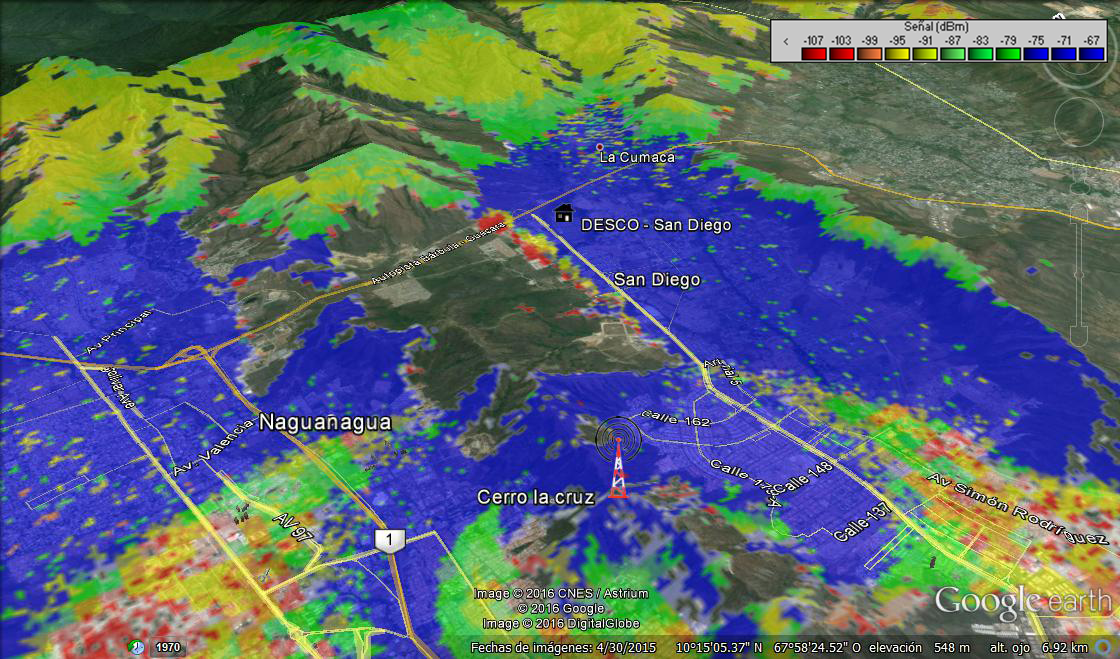
\includegraphics[width=0.53\linewidth]{Cobertpolar2.png}
    \caption{Cobertura polar de la zona. Radio Mobile}
    \label{fig:p2}
\end{figure}

\chapter{Sistemas de protección}

\section{Sistema de puesta a tierra}
El aterrizaje o puesta a tierra consiste en la conexión intencional de una fase o conductor neutro a la tierra, con el propósito de controlar el voltaje a tierra o masa, dentro de límites predecibles\cite{howell82}. Ante una descarga atmosférica o un corto circuito, sin tierra física, las personas estarían expuestas a una descarga eléctrica, los equipos tendrían errores en su funcionamiento. Si las corrientes de falla no tienen un camino para disiparse, por medio de un sistema de conexión correctamente diseñado, entonces éstas encontrarían caminos no intencionados que podrían incluir a las personas\cite{montiel2005}.

El suelo, al igual que cualquier material conductor eléctrico, se opone al paso de la corriente eléctrica y ofrece una resistencia, el factor más importante de la resistencia de la tierra es la resistividad del suelo, por lo que es un requisito conocerla para calcular y diseñar un sistema de puesta a tierra. La medición de la resistividad está sujeta al promedio de varias mediciones que deben ser realizadas, ya que los suelos no son uniformes en las diferentes capas que lo componen. La IEEE\cite{howell82} indica que este cálculo ha sido simplificado a una fórmula aplicable para la mayoría de los casos, para una tierra de resistividad uniforme $\rho \Omega \cdot cm$ 

\begin{equation}
    R_{g}(rod) = \frac{\rho (\Omega \cdot cm)}{335 cm} \Omega
\end{equation}

Cabe destacar que la resistividad de los suelos puede ser reducida en cualquier lugar de un $15$ a un $90 \%$ por tratamiento químico (Dependiendo del tipo de textura del suelo) entre los químicos adecuados para este propósito, se encuentran el Cloruro de Sodio, Sulfato de Magnesio, Sulfato de Cobre y el Cloruro de Calcio. La sal común y el sulfato de magnesio son los más comúnmente usados.

A propósito de los métodos de puesta a tierra de sistemas de telecomunicaciones,  indica que, debido a las altas frecuencias involucradas, se requiere en este caso un diseño diferente para la malla de puesta a tierra. Siendo su objetivo el maximizar la cantidad de conductor en la vecindad inmediata de la estructura. Para la DESCO-San Diego se propone entonces un diseño similar al mostrado en la Fig. \ref{fig:pt}.  En este esquema\cite{bautista2015}, se deberán instalar largos alambres delgados en forma radial desde el mástil de comunicación, colocados a una pequeña profundidad usando la técnica de arado. 

\begin{figure}[h]
    \centering
    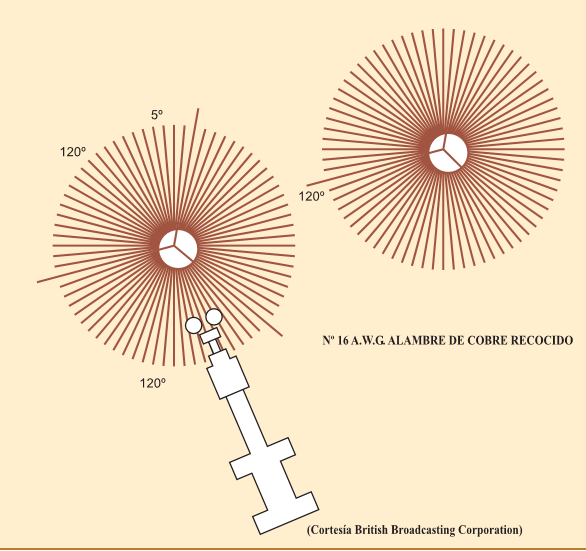
\includegraphics[width=0.5\textwidth]{fig14.png}
    \caption{Malla de puesta a tierra, sistemas de RF. M. Bautista}
    \label{fig:pt}
\end{figure}

El detalle de las barras horizontales de la figura \ref{fig:pt} se muestra en la siguiente figura:

\begin{figure}[h]
    \centering
    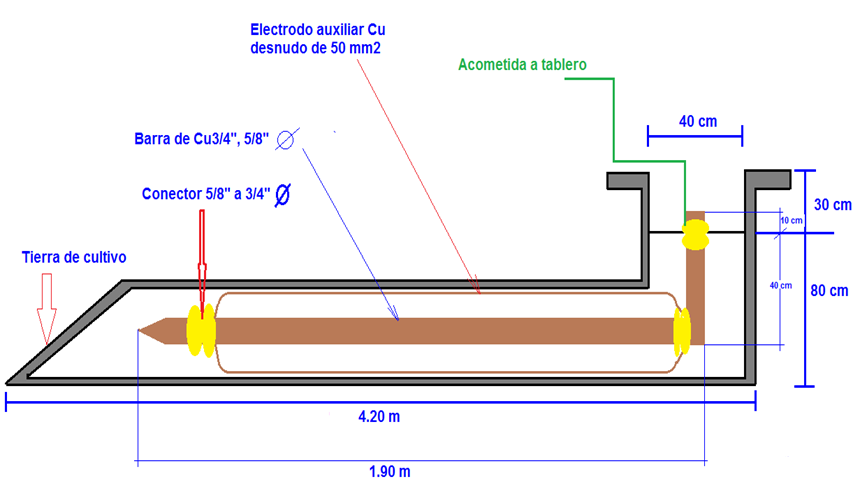
\includegraphics[width=0.5\textwidth]{fig15.png}
    \caption{Barra horizontal de aterrizamiento. M. Bautista}
    \label{fig:15}
\end{figure}

Se recomienda que en la instalación de las varillas horizontales se utilice \textit{cemento conductivo}, el mismo debe ser vertido alrededor del conductor y tirado a lo largo de la zanja horizontal. Éste absorberá la humedad del suelo circundante y se endurece para convertirse en un conductor sólido, la superficie del electrodo aumentará considerablemente, la resistencia a tierra se reducirá sustancialmente obteniendo como resultado una menor impedancia.

\subsection{Presupuesto}
De acuerdo a los esquemas \ref{fig:pt} y \ref{fig:15} serán necesarias 24 varillas de cobre de 5/8 pulgadas de diámetro y cemento conductivo suficiente para la instalación de las varillas, consultando los sitios web \href{http://www.mercadolibre.com.ve/}{MercadoLibre Venezuela} y \href{https://www.alibaba.com/}{Alibaba} se obtienen los precios estimados para el 10 de noviembre de 2016.

\begin{table}[h]
    \centering
    \begin{tabular}{|c|c|c|}
        \hline
        \cellcolor{gray75} \textbf{Material} & \cellcolor{gray75} \textbf{Cantidad} & \cellcolor{gray75} \textbf{Costo/Unidad ($ Bs $)} \\ \hline
        Barras De Cobre De 5/8 & 72 U & 12.000 \\ \hline
        Cemento Conductivo & 1 Ton & 65.788.78 \\ \hline
    \end{tabular}
    \caption{Presupuesto para implementación de malla de puesta a tierra}
    \end{table}

\section{Protección contra descargas}
 La protección contra descargas atmosféricas es esencial para el resguardo de edificios, lineas de transmisión y equipos eléctricos\cite{howell82}. La acumulación de electricidad estática  en equipos, material manipulado o procesado y en el personal operario, introduce una seria amenaza potencial en cualquier sitio donde estén presentes líquidos explosivos, gases, polvo o fibras, la descarga de una acumulación de electricidad estática desde un objeto hasta la tierra u otro objeto cargado de distinto voltaje puede ser la causa de un incendio o una explosión si tiene lugar en presencia de materiales inflamables o ante la combinación de aire y vapores combustibles, estas explosiones o incendios pueden causar lesiones al personal que opera el equipo de comunicaciones o incluso su muerte, sin contar las pérdidas económicas millonarias que supone el deterioro de los equipos y estructuras afectadas.
 
  Para conocer la frecuencia de eventos atmosféricos en la zona DESCO-San Diego, se recurre a estudios estadísticos  derivados en la elaboración de un mapa Ceráunico\footnote{Un mapa ceráunico es un tipo de mapa geográfico que representa a una zona o país para determinar el nivel de riesgo de rayos} de acuerdo al cual, el estado Carabobo experimenta, en promedio, alrededor de $2 \, descargas/Km^{2}/año$. 
  
  Se recomienda instalar un pararrayos Frankiln, cuya implementación básica  está constituída por:

\begin{itemize}
    \item Una varilla captadora, junto con su mástil.
    \item Uno o dos bajantes.
    \item Un desconectador por bajante para la comprobación de la resistencia de la estructura.
    \item Un elemento protector contra golpes en los dos últimos metros del bajante conductor.
    \item Una toma de tierra por bajante.
    \item Unión equipotencial de las tomas de tierra y circuito general de tierras.
\end{itemize}

\begin{figure}[h]
    \centering
    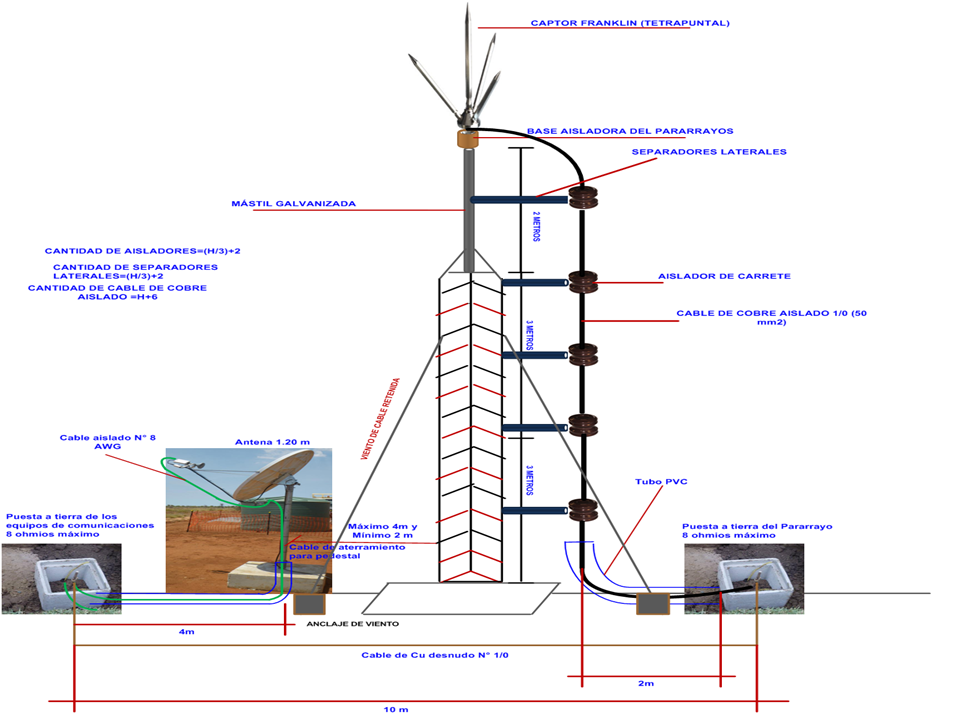
\includegraphics[width=0.5\textwidth]{fig11.png}
    \caption{Sistema de protección recomendado contra descargas eléctricas. M. Bautista}
    \label{fig:11}
\end{figure}

El sistema mostrado en la figura \ref{fig:11} está constituído por un pararrayos Franklin, un mecanismo de derivación constituído por un cable de cobre, aislado de la torre por carretes cerámicos, de 50 mm$^{2}$ el cual conecta al terminal aéreo con una serie de varillas de aterrizaje cuya longitud y separación dependerán principalmente del área disponible alrededor de la torre; como regla de pulgar, la distancia entre dos electrodos debe ser como mínimo el cuádruple de su longitud; por otro lado, en sistemas donde se requiera obtener resistencias eléctricas muy bajas y exista espacio suficiente, se debe maximizar esta distancia, para evitar que se susciten resistencias mutuas entre las varillas \cite{bautista2015}.

\begin{figure}[h]
    \centering
    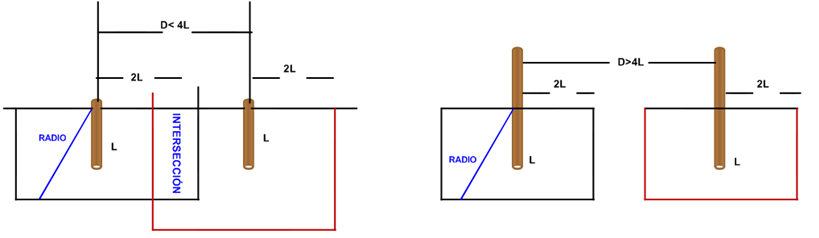
\includegraphics[width=0.5\textwidth]{fig12.png}
    \caption{Separación entre las varillas de puesta a tierra. M. Bautista}
    \label{fig:12}
\end{figure}

\subsection{Presupuesto}
El sistema de protección contra descargas eléctricas requerirá del uso de un terminal aéreo (Punta Franklin), más de 18 metros de conductor de cobre de 50 mm$^{2}$ 6 aislantes de carrete y 2 metros de tubería PVC para conexiones eléctricas, consultando el sitio web \href{http://alibaba.com}{Alibaba} se obtienen los precios estimados para el 10 de noviembre de 2016.

\begin{table}[h]
    \centering
    \begin{tabular}{|c|c|c|}
        \hline
        \cellcolor{gray75} \textbf{Material} & \cellcolor{gray75} \textbf{Cantidad} & \cellcolor{gray75} \textbf{Costo/Unidad ($ Bs $)} \\ \hline
        Punta Franklin & 1 U & 38.000 \\ \hline
        Cable de Cobre 50 mm$^{2}$  & 25 m & 328.94 \\ \hline
        Aislante de Carrete & 6 & 600 \\ \hline
        Tubo PVC eléctrico & 2m & 950 \\ \hline
    \end{tabular}
    \caption{Presupuesto para implementación de malla de puesta a tierra}
\end{table}

\chapter{Canalizaciones}
\section{Diseño de la torre de telecomunicaciones}
La altura de la torre requerida para el proyecto (5 metros $\approx$ 16.4 pies) y el área limitada disponible en el espacio DESCO San Diego sugieren que la alternativa más adecuada es un poste hexagonal de 8 metros, debe considerarse que parte de la longitud del poste deberá ser fijado en la tierra para garantizar la estabilidad de la estructura.

La selección del tipo de torre obedece a criterios físicos (Disponibilidad de espacio), económicos (presupuesto disponible) y operativos (tipo de servicio a prestar y número de antenas requeridas)\cite{freeman2006radio}; existe una relación inversa entre la huella de la torre y su costo; entre más reducida sea la primera, mayor será el segundo, en consecuencia, de puede deducir que la torre monopolo es la más costosa, al presentar una huella mínima; en contraposición, la antena venteada es la más costosa pero la que  requiere de una mayor área libre, disponible para su instalación. 

Considerando la altura reducida necesaria para la implementación del enlace punto-punto entre DESCO y el Cerro La Cruz, se considera suficiente el uso de un poste metálico de al menos 5 metros de altura. A continuación se presenta un \href{http://articulo.mercadolibre.com.ve/MLV-462232615-postes-hexagonal-600-m-_JM}{presupuesto} del poste que cumple con tales características 

\begin{table}[h]
    \centering
    \begin{tabular}{|c|c|c|}
        \hline
       \cellcolor{gray75} \textbf{Modelo} & \cellcolor{gray75}\textbf{Altura (Metros)} & \cellcolor{gray75}\textbf{Precio $Bs$} \\ \hline
        Poste Hexagonal de Acero & 6 & 94.000 \\ \hline
        Poste Hexagonal de Acero & 8 & 126.400  \\ \hline
        Poste Hexagonal de Acero & 10 & 182.000  \\ \hline
    \end{tabular}
    \caption{Presupuesto de Construcción de Torres de Comunicaciones.
     \textit{Fuente: MercadoLibre Venezuela. 10/11/2016}}
     \label{tab:costorre}
\end{table}

\section{Instalación de tubería subterráneas}
 A continuación se describe el proceso para la instalación subterránea de la tubería PVC por la cual se extenderá el cable UTP que permitirá conectar la antena con el rack.
 
\subsection{Diseño de las tuberías PVC}
La longitud aproximada de la ruta es de 20m y considerando que los tubos de PVC tienen una medida estándar de 3m, se requieren como mínimo 6 unidades.
 
Adicionalmente se deben incluir los elementos para hacer las conexiones de los tubos y a su vez 4 codos para realizar las curvaturas necesarias que permitan la extensión de la tubería a 45cm de profundidad. La razón por la cual se profundizará dicha tubería a 45cm por debajo de la superficie es tomando en cuenta las normas COVENIN, donde se especifica que la profundidad mínima para canalizaciones subterráneas es de 45cm. Es importante el uso de un buen pegamento para el empalme de las tuberías y asegurar que queden bien selladas las uniones para evitar que haya presencia de humedad en la misma.

 Como se trata de un área despejada, se eligió la ruta más corta entre los puntos inicial y final para llevar las conexiones desde la antena receptora hasta el suiche principal. En la imagen siguiente se ilustra la ruta sugerida para la tubería subterránea.

\begin{figure}[h]
    \centering
    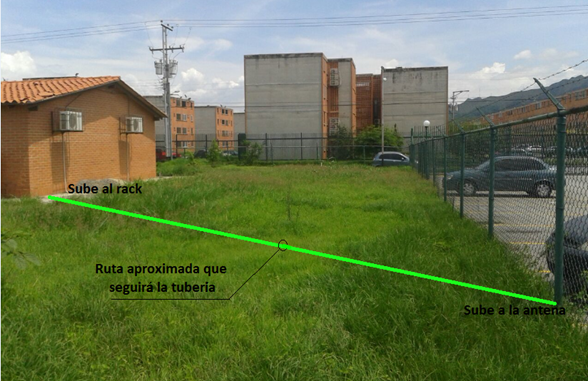
\includegraphics[width=0.6\textwidth]{Si1.png}
    \caption{Ruta subterránea sugerida para la tubería PVC.}
    \label{fig:frog1}
\end{figure}


\subsection{Diseño de la zanja o bancada para la ubicación de la tubería}
Para ello se revisaron las recomendaciones indicadas en el Código Eléctrico Nacional y en las normas de CANTV las cuales hacen referencia a las normas CADAFE sobre el diseño de bancada para colocación de tuberías subterráneas. En este caso, el diseño requerido es de una bancada B1- $\Phi$3/4, colocando la tubería a una profundidad mínima de 45cm sobre la rasante del terreno y un ancho mínimo de 30cm. 

\begin{figure}[h]
    \centering
    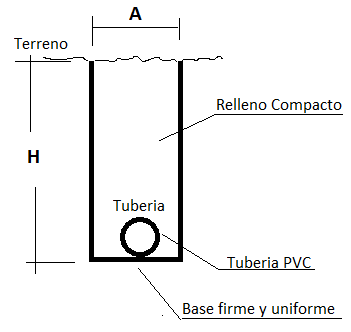
\includegraphics[width=0.4\textwidth]{Si3.png}
    \caption{Tubería Subterránea.}
    \label{fig:frog2}
\end{figure}

Al momento de construir la bancada se debe lograr construir una base y unas paredes laterales uniformes y firmes donde descansará la tubería y finalmente compactar con un buen relleno tal como muestra la Fig. \ref{fig:frog2}. Para el relleno puede utilizarse gravilla fina y una capa ligera de cemento en la superficie para asegurar el buen resguardo de la tubería y evitar fracturarla con algún tipo de relleno pesado.

La cantidad del cableado necesario (por exceso) para realizar la conexión que va desde la antena hasta el switch es de 25 metros, tomando como referencia las distancias calculadas para la canalización a utilizar. De este modo, se establece una cantidad cable de guarda aproximada de 1,5 metros, la conexión se realizara por medio de conectores RJ-45 en donde para la realización de la implementación se requieren de 4, sugiriendo la adquisición de 6 previniendo la necesidad de alguno más a causa de cualquier eventualidad.

La figura \ref{fig:frog3} muestra un esquema completo sobre la implementación a utilizar.
\begin{figure}[h]
    \centering
    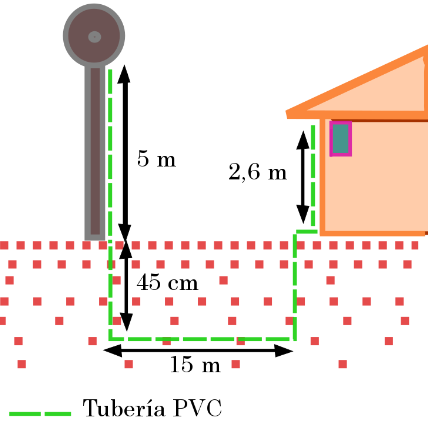
\includegraphics[width=0.4\textwidth]{tulo.png}
    \caption{Esquema final sugerido en el diseño a implementar}
    \label{fig:frog3}
\end{figure}

\section{Presupuesto}
A continuación se presenta la siguiente tabla con los materiales que se requieren para la implementación con su respectivo precio en Bolivares.

\begin{table}[h]
    \centering
    \begin{tabular}{ | c | c | c | c | }
    \hline
    	\cellcolor{gray75}\textbf{Materiales} & \cellcolor{gray75}\textbf{Costos Bs} & \cellcolor{gray75}\textbf{Unidades}  \\ \hline
    	Tubos PVC 3/4 & 260Bs & 7  \\ \hline
    	Conexiones PVC & 200Bs & 7 \\ \hline
    	1Abrazaderas de Acero Inoxidable & 310Bs& 10  \\ \hline
    	Pegamento para PVC(320Oz) & 2.250Bs.&    2\\ \hline
        Conectores RJ-45 & 50Bs & 6   \\ \hline
    	CABLE UTP Cat5 & 230Bs/metro & 25metros  \\ \hline
    \end{tabular}
    \caption{Tabla de costos.}
    \label{tab:cost3}
\end{table}

\chapter{Infraestructura de comunicaciones en\\ Cerro la Cruz}
Para el despliegue de comunicaciones entre DESCO-San Diego y DIMETEL, mediante un enlace en Cerro la Cruz, es necesario colocar la antena Rocket M5 Titanium en la torre ventada propiedad de la Universidad de Carabobo. Se deben tomar todas las previsiones posibles al momento de utilizar los tie-wraps en la puesta de el cable ethernet sobre la torre.

Ya que existe linea de vista entre los dos puntos, ambas antenas se deben posicionar con los ángulos de elevación y azimut descritos en el capitulo \ref{chap:radio} creando el enlace, la antena del punto Cerro la Cruz cuenta con una apertura de $120^{\circ}$, este se realizará a una frecuencia de 5.7GHz, que se encuentra dentro de su rango de operación que es 5170 - 5825 MHz, tiene un alcance de +50km,y una potencia de salida de 27 dBm, las especificaciones de potencia de transmisión y recepción van a depender de la velocidad de el enlace y el esquema de modulación seleccionado, lo cual depende directamente de las interfaces presentes en los equipos de la caseta.

Adentrando un poco más en los materiales a utilizar, especificaciones y presupuestos aproximados para realizar dicha implementación, se proponen dos casos bastante efectivos, los cuales son:

\begin{enumerate}
    \item Caso A:
    Éste caso consiste básicamente en adquirir, los Tirrajes, conectores RJ-45 y el Cable UTP Cat5e Intemperie, considerando que éste último está diseñado para funcionar al aire libre, se podría implementar de una manera efectiva y económica, resaltando que dicho cable iría desde la antena hasta la base de la torre, utilizando precintos de plástico cada metro y luego desde éste punto de la torre hasta el cuarto de control. \textbf{TOTAL: 8.200 BsF.} 
    \begin{table}[h]
        \centering
        \scalebox{0.8}{\begin{tabular}{| c | c | c | c | }
         \hline
        \cellcolor{gray75}Material & \cellcolor{gray75}Cantidad & \cellcolor{gray75}Precio por unidad &\cellcolor{gray75} Precio total \\ \hline
         Cable UTP Cat 5e Intemperie Color Negro. & 30 m & 230 BsF & 6900BsF \\ \hline
         Tirrajes (Tie Wraps) 30cm X 5mm Color Negro. & 50 pzas & 1200 BsF & 1200BsF \\ \hline
         Conectores RJ-45 & 2 pzas & 50 BsF & 100 BsF \\
         \hline
       \end{tabular}}
       \caption{Lista de precios y elementos}
       \label{tab:4}
    \end{table}
    \newpage
    \item Caso B:
    El siguiente caso consiste en adquirir, los Tirrajes, conectores RJ-45, tubos PVC y el Cable UTP Cat 5e Intemperie, considerando para éste caso un mayor cuidado sobre el cable, se colocará un tubo PVC desde la antena hasta la base de la torre y dentro de dicho tubo iría el cable UTP cat 5e, además de ir colocando precintos de plástico cada metro para unir dicho tubo con la torre, lográndose una implementación totalmente segura hacia cualquier tipo de daño que le puedan realizar al cable, pero resulta un poco más costosa que la anterior, finalmente desde la base de la torre hasta el Cuarto de Control ya está la existencia de una tubería garantizando la seguridad y el cuidado de dicho cable, alcanzándose un buen desempeño de todo el sistema. \textbf{TOTAL: 11.440 BsF.} 
    \begin{table}[h]
        \centering
         \scalebox{0.8}{\begin{tabular}{| c | c | c | c | }
        \hline
        \cellcolor{gray75}Material & \cellcolor{gray75}Cantidad & \cellcolor{gray75}Precio por unidad &\cellcolor{gray75} Precio total \\ \hline
         Cable UTP Cat 5e Intemperie Color Negro. & 30 m & 230 BsF & 6900BsF \\ \hline
         Tubo PVC 3/4'' & 12 m & 270 BsF & 3240BsF \\ \hline
         Tirrajes (Tie Wraps) 30cm X 5mm Color Negro. & 50 pzas & 1200 BsF & 1200BsF\\ \hline
         Conectores RJ-45 & 2 pzas & 50 BsF & 100 BsF \\
        \hline
        \end{tabular}}
        \caption{Lista de precios y elementos}
         \label{tab:5}
    
    \end{table}
\end{enumerate}
En la Fig. \ref{fig:tower} se observa la torre sobre la caseta de Cerro la Cruz, los vientos se encuentran en los extremos de los tramos de 3mts, como la longitud de la torre es de 9mts esta consta de tres vientos que la sujetan, todo esto con el fin de que la torre esté firmemente soportada a su centro de masa. 
\begin{figure}[h]
    \centering
    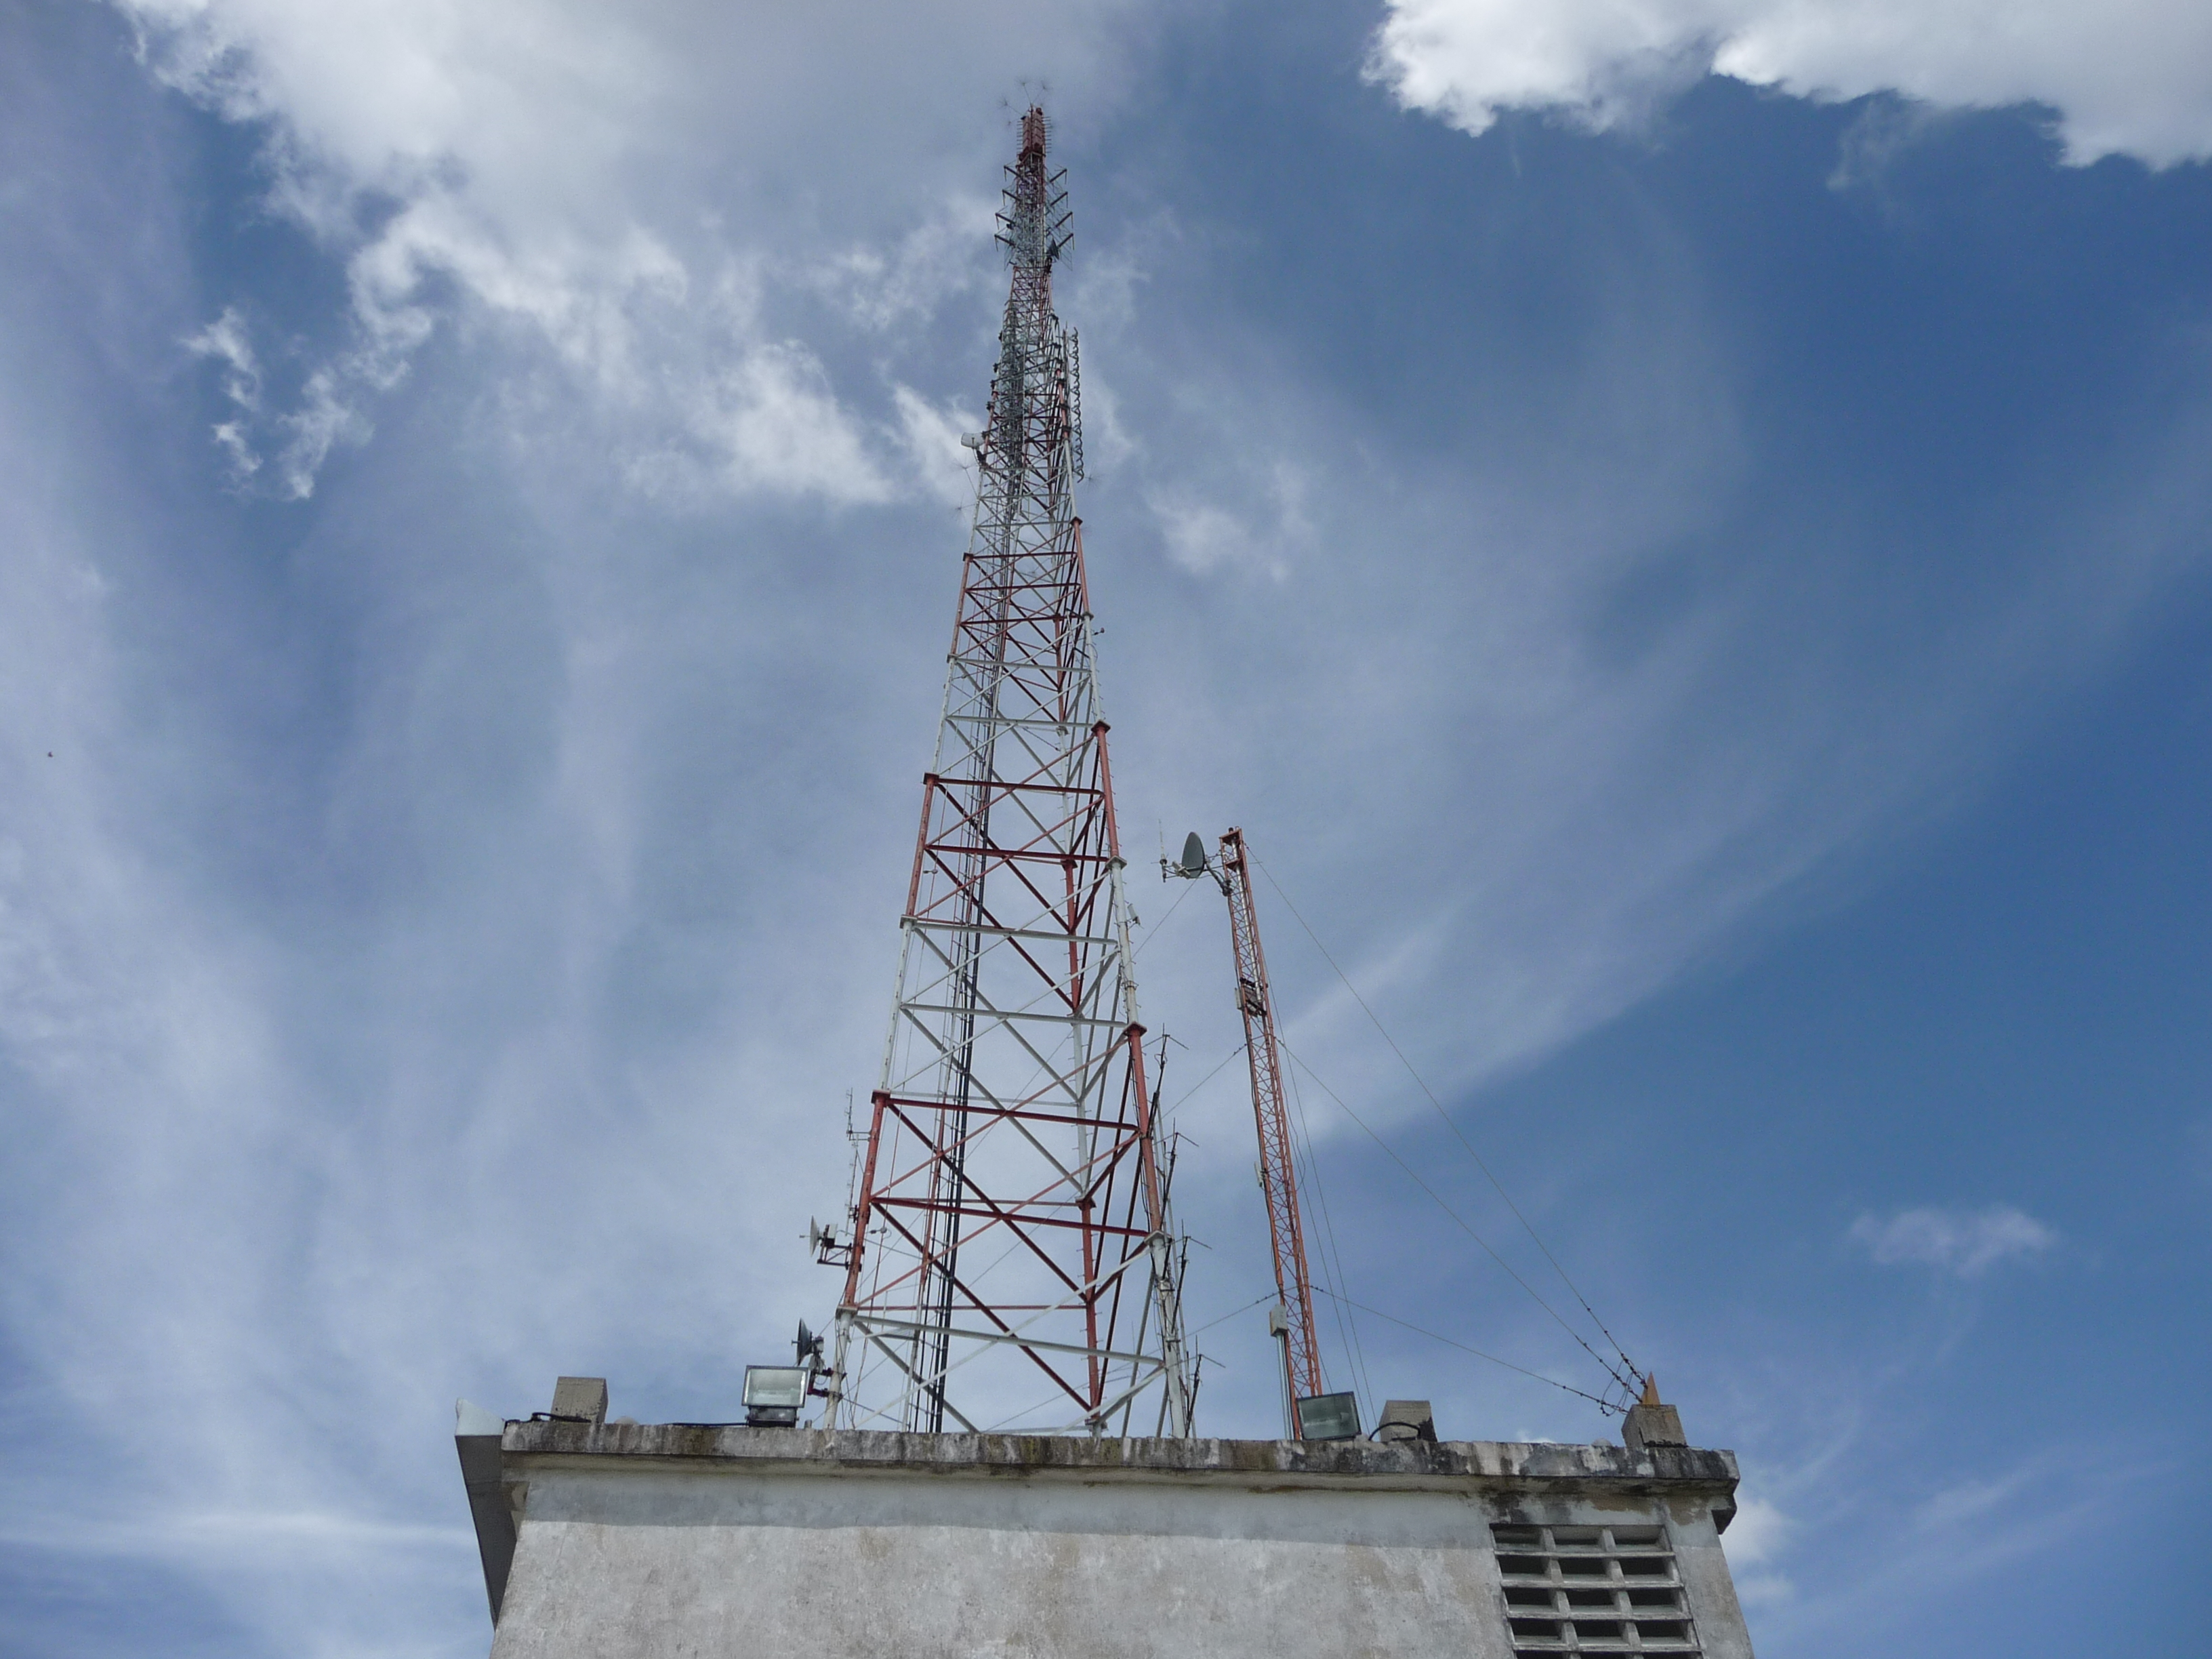
\includegraphics[width=0.728\textwidth]{cerro_la_cruz_1.jpg}
    \caption{Torre ventada sobre caseta de la Universidad de Carabobo en Cerro la Cruz.}
    \label{fig:tower}
\end{figure}

\chapter{Cableado estructurado}
\begin{figure}[h]
    \centering
    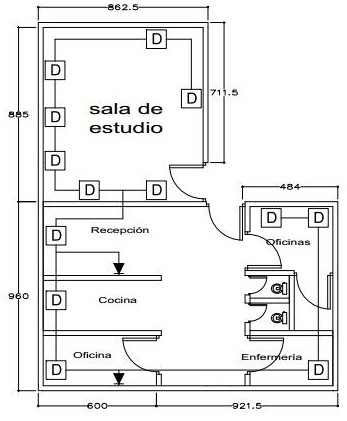
\includegraphics[width=0.85\linewidth]{cableado.png}
    \caption{Cableado estructurado del recinto. Los simbolos D son conexiones de datos, y los delta puntos de acceso telefónico}
    \label{fig:cab}
\end{figure}
Al momento de realizar la implementación de la red interna en los distintos espacios de la DESCO, se debe tomar en consideración la disposición de los equipos sede red, como el suiche y los distintos puntos de acceso, ya que el suiche cuenta con 24 puertos será la cantidad máxima de puntos a colocar.

\chapter{Diseño de la topología de red}
\begin{figure}[h]
    \centering
    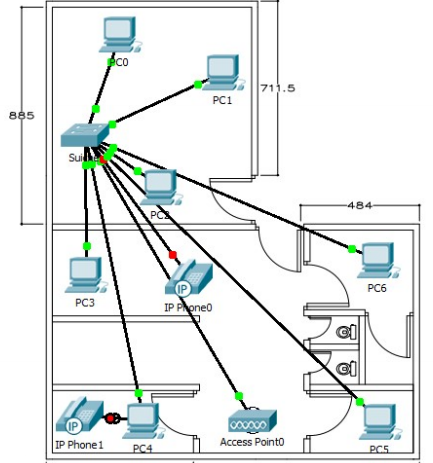
\includegraphics[width=1\linewidth]{topo.png}
    \caption{Topología de red. Cisco Packet Tracer}
    \label{fig:topo}
\end{figure}

Al ser la dependencia DESCO-San Diego un recinto de medianas dimensiones se consideró que la mejor distribución de la red es una topología en estrella. De este modo, las conexiones a los distintos equipos de red son repartidas mediante un suiche central.

\chapter{Catalogo de equipos}
A continuación se listan los equipos mínimos necesarios para tener la red operativa, no se toman en cuenta los precios de los equipos. 
\begin{table}[h]
    \centering
    \begin{tabu}{|C{5cm}|C{5cm}|}
        \hline \cellcolor{gray75} \textbf{Equipo}  &  \cellcolor{gray75} \textbf{Características} \\
         \hline suiche Cisco Linksys SR224 &   24 puertos, conexión Fastethernet 10/100\\
         \hline regleta  Wireplus & 8 tomas, 15 amperios \\
         \hline Patch Panel Hubbell & 24 puertos\\
         \hline Ups Apc Br1000g  & 1000 VA\\
         \hline Rack de pared 4U-19 & Soporte para equipos de telecomunicaciones\\
         \hline Router Tp-Link & 2.4 y 5.1 Ghz, 3 antenas\\
         \hline Barra Copperweld ce cobre & 5/8 pulgadas\\
         \hline 
    \end{tabu}
\end{table}

\section{Dispositivos Recomendados}
\begin{enumerate}

\item Se seleccionó un Suiche de 24 puertos, actualmente la sede no amerita de tal cantidad de puntos de red disponible pero es probable un incremento en los próximos años en la sala principal del recinto.
\item Para el suiche elegido se adiciona un patch panel de 24 puertos para cableado UTP categoría 5E.
\item Una regleta  de 8 puertos que será ubicada en el mismo rack para la alimentación de los dispositivos.
\item Un UPS que cumple la función de proteger  de sobrecargas y respaldar por un máximo de 15 minutos los dispositivos conectados.
\item RACK de 4U.
\item Se ubico un Router inalámbrico para el personal y usuarios de las instalaciones accedan a la red con sus dispositivos móviles o laptops.
\item Barra de puesta a tierra para protección de los equipos ante descargas eléctricas.
\end{enumerate}
%%%%%%%%%%% BIBLIOGRAFÍA %%%%%%%%%%%%%%%%%%%%%%%%%%%%%%%%%%%%%%%%
\clearpage
\renewcommand*{\bibfont}{\scriptsize}
\pagestyle{plain}
\printbibliography

\end{document}
